% Chapter X

\chapter{Boiling Bubble Dynamics} % Chapter title

\label{ch:bub_dyn} % For referencing the chapter elsewhere, use \autoref{ch:name} 

%----------------------------------------------------------------------------------------

\section{Introduction}

Boiling bubble parameters are playing an important role in the Heat Flux Partitioning models. For instance, the evaporation heat flux $\phi_{e}$ is directly proportional to the bubble lift-off radius $R_{lo}$ \ref{eq:phie_KP} while the quenching heat flux $\phi_{q}$ depends on the wall area visited by a bubble $A_{q,1b}$ (Eq. \ref{eq:phiq_Basu}) which depends on the bubble sliding length $l_{sl}$, departure raidus $R_{d}$ and lift-off radius $R_{lo}$.

\subsection{Experimental Insights}

Consequently, many experimental investigations have been conducted to further understand the behavior of nucleated bubbles on a wall while facing a liquid flow. In the case of vertical flow boiling, a typical bubble life cycle can be described as follows:

\begin{itemize}
\item Beginning of nucleation, growth while attached to the nucleation site ;

\item Detachment occurring at radius $R_{d}$, from which the bubble will start to slide and accelerate along the wall ;

\item Lift-off from the wall at radius $R_{lo}$ after sliding over a length $l_{sl}$.

\end{itemize}


This behavior has been supported by many experimental observations who clearly observed three stages (departure, sliding, lift-off) both at low pressure (Maity \cite{maity_effect_2000}, Situ \cite{situ_bubble_2005}, Thorncroft \cite{thorncroft_experimental_1998}, Prodanovic \cite{prodanovic_2006}, Chen \cite{chen_prediction_2012}, Ren \cite{ren_development_2020}, etc.) and high pressure (March \cite{march_1990}, Kossolapov \cite{kossolapov_experimental_2021}). Altogether, those works cover various flow conditions and operating fluids which insist on the generality of this bubble behavior in vertical flow boiling. Examples from the literature of visualizations of bubble sliding at atmospheric and high pressure are reproduced on Figure \ref{fig:slide_exp_vis}.

\begin{figure}[H]

\begin{center}

\subfloat[Bubble sliding visualized and adapted from Maity \cite{maity_effect_2000} at atmospheric pressure.]{
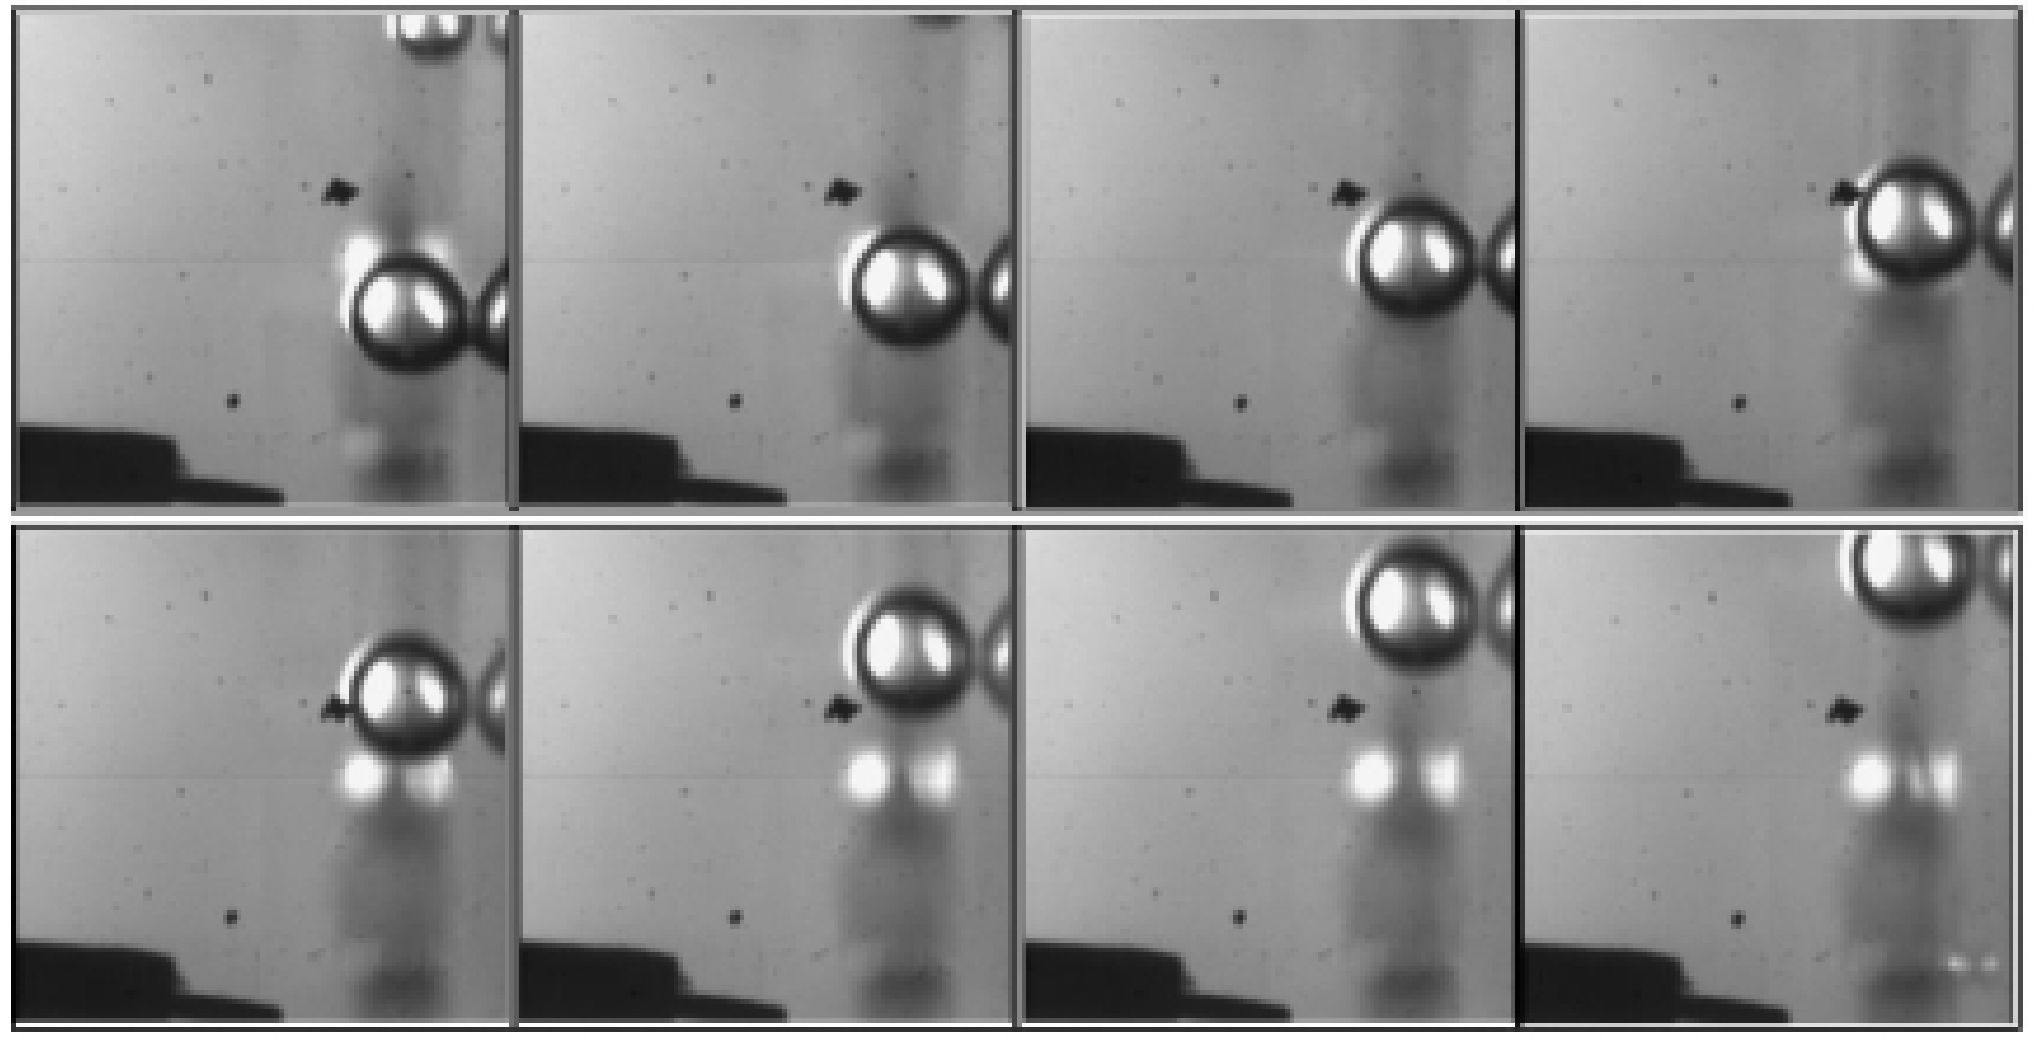
\includegraphics[width=0.6\linewidth]{img/forces/slide_maity.png}
} 
\\
\subfloat[Bubble sliding visualized and adapted from Kossolapov \cite{kossolapov_experimental_2021} at higher pressure.]{
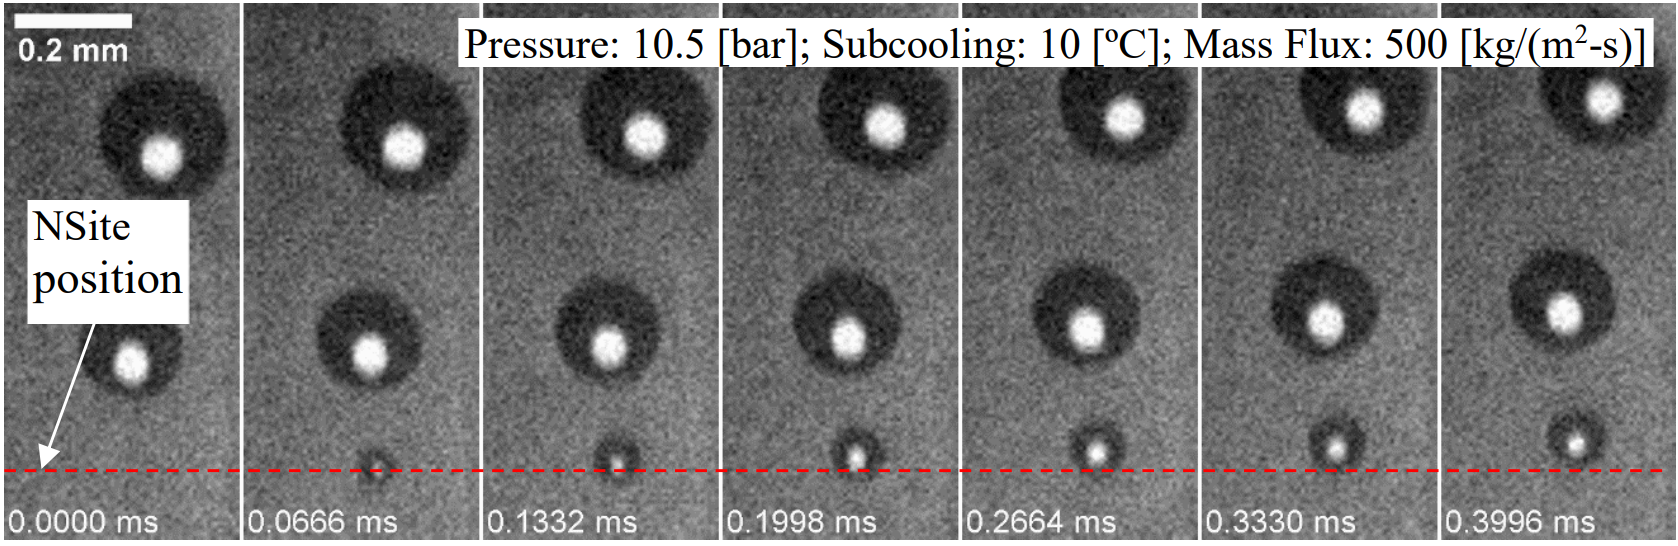
\includegraphics[width=0.6\linewidth]{img/forces/slide_koss.png}
} 

\end{center}

\caption{Visualization of bubble sliding at various pressures.}
\label{fig:slide_exp_vis}
\end{figure}


The bubble sliding process has also been thermally studied to quantify its impact over the wall heat transfer. Estrada-Perez \etal \cite{estrada-perez_time-resolved_2018} observed the significant thermal impact of sliding bubbles footprints. Kossolapov \cite{kossolapov_experimental_2021} also investigated the sliding of boiling bubbles and measured the magnitude of the transient heat transfer induced by the disruption of the liquid thermal boundary layer in the bubble's wake. Typical experimental observations from those works a reproduced on Figure \ref{fig:slide_thermal_exp}

\begin{figure}[H]

\begin{center}
\subfloat[Instantaneous and time-averaged wall temperature in boiling regime visualized and adapted from Estrada-Pérez \etal \cite{estrada-perez_time-resolved_2018}.]{
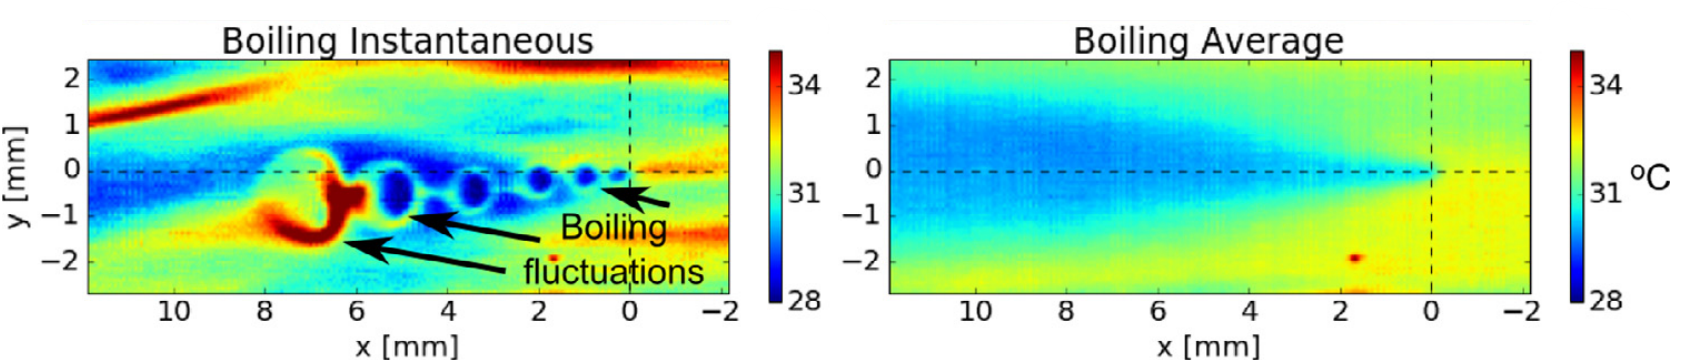
\includegraphics[width=0.8\linewidth]{img/forces/slide_thermal_estrada.png}
}
\\
\subfloat[Transient conduction induced by sliding bubbles visualized and adapted from Kossolapov \cite{kossolapov_experimental_2021}.]{
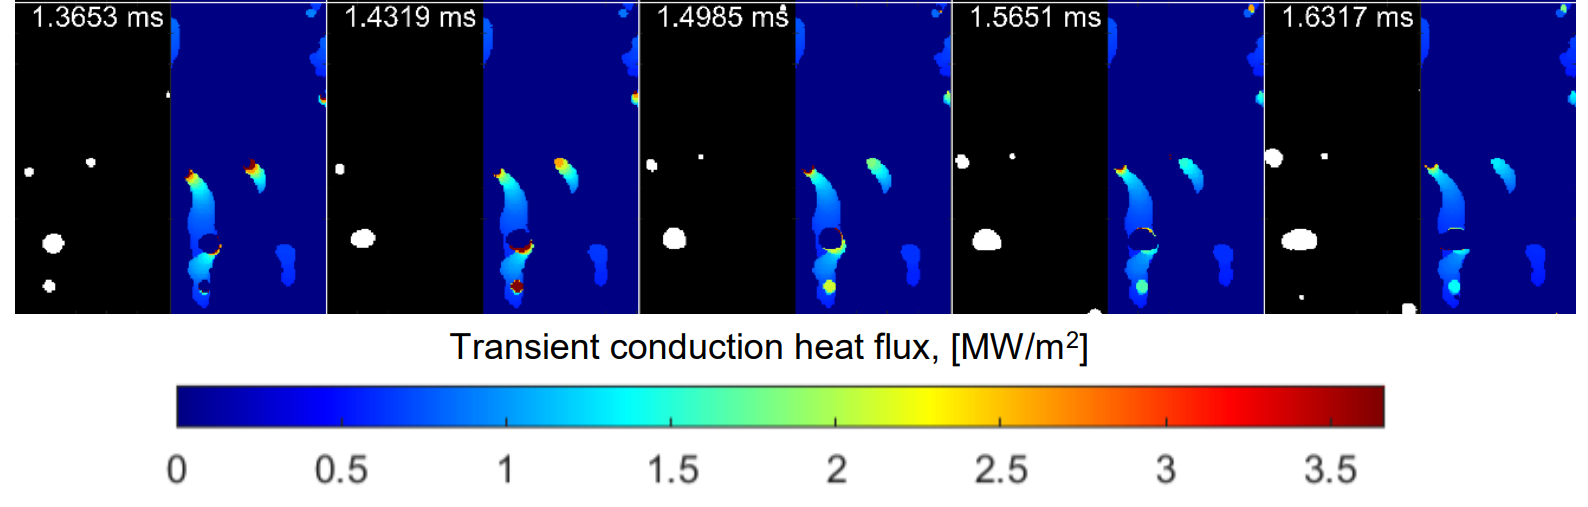
\includegraphics[width=0.8\linewidth]{img/forces/slide_thermal_koss.png}
}
\end{center}

\caption{Visualization of bubble sliding thermal impact.}
\label{fig:slide_thermal_exp}
\end{figure}


Those experimental observations highlight the significant magnitude of the transient heat transfer triggered by bubble movement on the wall that can represent up to 40\% of the total wall heat flux \cite{kossolapov_experimental_2021}. All the aforementioned observations are summed-up on Figure \ref{fig:sketch_bub_VFB}. 

\begin{figure}[H]
\centering
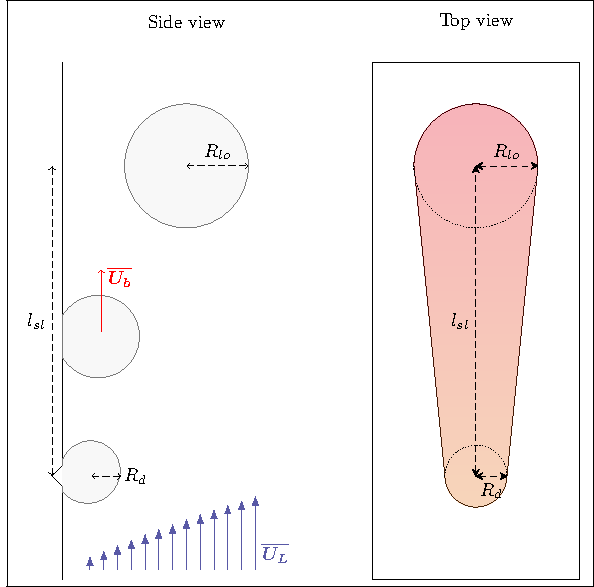
\includegraphics[width=0.65\linewidth]{img/forces/bub_life_VFB.pdf}
\caption{Sketch of a typical bubble lifetime in vertical flow boiling. Left depicts a typical side view of the heater with identification of departure, sliding and lift-off. Right depicts a top view of the heater, exhibiting the area that will undergo transient heat transfer.}
\label{fig:skecth_bub_VFB}
\end{figure}

Predicting the HFP in vertical flow boiling thus requires a descriptions of single bubble dynamics that includes accurate estimations of bubble departure and lift-off radiuses $R_{d}$ and $R_{lo}$ as well as bubble sliding velocity $\vect{U_{b}}$ to predict the sliding length $l_{sl}$.

\subsection{Existing Approaches}

Historically, first approaches to estimate the bubble diameter consisted of experimental-based correlations for pool boiling of horizontal surfaces through photographic studies. In those cases, departure from the nucleation site coincides with the bubble lift-off. Among the mainly used in HFP models and CFD, we can mention the law of Tolubinsky \& Kostanchuk (1970)\cite{tolubinsky_diam} which depends only on the local liquid subcooling:

\begin{equation}
D_{lo} = D_{0} e^{-\Delta T_{L}}/{45},\ D_{0}=15\mathrm{mm}
\end{equation}

On the other hand, authors such as Cole \& Rosenhow (1968) proposed relationships including the influence of pressure through the the capillary length $L_{c}=\sqrt{\frac{\sigma}{g\parth{\rho_{L}-\rho_{V}}}}$:

\begin{align}
D_{lo} =& C L_{c} \parth{\frac{\rho_{L}c_{p,L}T_{sat}}{\rho_{V}h_{LV}}}^{5/4}\\
\nonumber C=&1.5\times 10^{-4}\ \text{for water and }4.65\times 10^{-4}\ \text{else}.
\end{align}

This equations provides a good trend for the evolution of bubble departure diameter with pressure as shown by Kossolapov \cite{kossolapov_experimental_2021}.

\npar

Later, \"Unal (1976)\cite{unal_maximum_1976} derived a correlation based on semi-analytical approach of the heat transfer mechanisms around a bubble to estimate its maximum diameter, including simultaneous influences of pressure, heater material, liquid velocity and subcooling:

\begin{align}
D_{lo}=&2.42\times 10^{-5} P^{0.709}\frac{a}{\sqrt{b\varphi}}\\
\nonumber a =& \frac{\Delta T_{w}\lambda_{w}}{2\rho_{V}h_{LV}\sqrt{\pi \eta_{w}} }\\
\nonumber b =& \frac{\Delta T_{L}}{2\parth{1-\rho_{V}/\rho_{L}}}\ \text{and}\ \varphi=\max{1\ ;\ \parth{\frac{U_{L}}{U_{0}}}^{0.47}},\ U_{0}=0.61~\mathrm{m/s}
\end{align}

\"Unal validated his law against several measurements from the literature covering pressures from 1 to 177 bars, liquid velocities from 0.08 to 9.15 m/s, subcoolings from 3 to 86K and heat fluxes from 0.47 to 10.64 MW/m\up{2}.


\begin{remark*}{}
The law of \"Unal is used in the HFP model of Kurul \& Podowski. It as also implemented in NEPTUNE\_CFD HFP and includes a correction of Borée \etal to avoid divergence in bubble diameter when reaching saturated conditions.
\end{remark*}

\npar

More recently, the several developments around HFP models has lead meany researchers to propose dedicated correlations for bubble departure or lift-off diameter. For instance, Basu \etal fitted expressions for $D_{d}$ and $D_{lo}$ on their own measurements:

\begin{align}
\frac{D_{d}}{L_{c}} =& 1.3 \sin{\theta_{s}}^{0.4}\crocht{ 0.13 e^{-1.75\times 10^{-4} \Re_{L,D_{h}}}+0.005 }\Ja_{w}^{0.45}e^{-0.0065\Ja_{L}}\\
%
\frac{D_{lo}}{L_{c}} =& 1.3 \sin{\theta_{s}}^{0.4}\crocht{ 0.2 e^{-1.28\times 10^{-4} \Re_{L,D_{h}}}+0.005 }\Ja_{w}^{0.45}e^{-0.0065\Ja_{L}}
\end{align}

They were validated for $14 \leq \Ja_{w} \leq 56$, $1 \leq \Ja_{L} \leq 138$, $0\leq \Re_{L,D_{h}} \leq 7980$ and $30\degree \leq \theta_{s} \leq 90 \degree$.


\begin{remark*}{}
Basu \etal use these own-developed laws in their HFP formulation to estimate bubble diameters.
\end{remark*}

\npar

Similarly, Kommajosyula gathered several bubble departure and lift-off diameter measurements from the literature and proposed the following reduced correlation:

\begin{align}
D_{d} = 18.9 \times 10^{-6} \parth{\frac{\rho_{L}-\rho_{V}}{\rho_{V}}}^{0.27} \Ja_{w}^{0.75} \parth{1+\Ja_{L}}^{-0.3} U_{L,bulk}^{-0.26}\\
D_{lo} = 1.2 D_{d}
\end{align}

\begin{remark*}{}
Although this law (used in Kommajosyula's HFP model) present coherent trends with flow conditions, the raw presence of $U_{L,bulk}$ in the expression is questionable because:

\begin{itemize}
\item The relationship is not dimensionless and the constant $18.9 \times 10^{-6}$ must be in m\up{1.26}.s\up{-0.26} ;
\item The negative exponent will yield diverging values when reaching pool boiling conditions, which is not physically coherent.
\end{itemize}
\end{remark*}


However, explicit correlations include limited range of application depending on the flow conditions over which they have been established. To overcome this drawback and try to come up with more generalized models, researchers have developed Mechanistic Models based on a force-balance approach to precisely depict the external efforts experienced by the growing bubble. The goal is to compute the sum of the forces applied to the bubble over its growing time and to detect departure and lift-off events using associated criteria such as a change in the force balance sign.




\section{Bubble Force Balance in Vertical Flow Boiling}

One of the firstly introduced model of this kind was proposed by Klausner \etal in 1993 \cite{klausner_vapor_1993} validated on horizontal flow boiling of refrigerant. It was followed by several subsequent works among which Van Helden \etal \cite{van_helden_forces_1995} who assessed forces coefficients using injected air bubbled in a vertical flow or Thorncroft \cite{thorncroft_bubble_2001} who compared his predictions with vertical and horizontal flow boiling of R113. Later, Duhar \& Colin \cite{duhar_dynamics_2006} validated a force balance on bubbles created by air injection in a shear flow. Sugrue \etal \cite{sugrue_experimental_2014} studied water flow boiling with varying surface orientation with their results used by Mazzocco \etal \cite{mazzocco_reassessed_2018} who validated his model against several low pressure measurements from literature. For more recent works, we can mention Ren \etal \cite{ren_development_2020} who used own measurements of vertical flow boiling of water up to 5 bar. Each of those models proposed different upgrades and modifications to the force balance depending on the aimed experimental conditions.

Unfortunately, all the aforementioned works were validated using low pressure experiments due to the lack of pressurized measurements in the literature. In addition, the common use of several empirical parameters makes it difficult to reach a general validation of those models. The present study, anchored in this framework, aims to propose an update of the bubble force balance for vertical boiling flows with a reduced empiricism and to study the sliding phenomenon by both conducting a non-dimensional analysis of the departure by sliding as well as predicting the subsequent departure diameter and sliding velocity of the bubble. By focusing on the force balance parallel to the wall, the approach is validated against measurements in various flow conditions, including pressure up to 40 bar thanks to the recent work of Kossolapov \cite{kossolapov_experimental_2021}. This ensures an encouraging generality of the proposed approach compared to previous models.


In this section, we wish to detail expressions of the different forces experienced by the bubble and to compare their magnitude in order to assess which will be predominant in the departure and lift-off process.

\subsection{Bubble shape : Geometrical definitions}

\label{subsec:geom_bub}

In order to clearly express each of the considered forces, assumptions regarding the shape of the bubble nucleating at the wall are needed.

\npar

Here, we assume that the bubbles will mostly have the shape of a truncated sphere with respect to the contact angle $\theta_{s}$ (Fig. \ref{fig:bub_shape}), being a thermophysical property of the fluid and the  wall. This assumption can thoroughly be discussed since many experimental measurements and visualizations have shown that in the case of low pressure boiling, bubbles tend te be strongly deformed depending on the flow conditions (\textsc{Maity}, \textsc{Estrada-Pérez} \etal, etc.) thus casting doubts on spherical or quasi-spherical hypotheses.

\npar
On the other hand, experiments conducted by \textsc{Kossolapov} found that in vertical flow boiling, increasing pressure leads to smaller and less deformable bubbles. Thus, supposing a truncated spherical shape could be relevant to model nucleating bubbles on a heater surface. Moreover, working on highly deformed bubbles would undoubtedly imply complicated calculations and extra parameters to account for.

\textsc{Kossolapov}'s measurements also concluded that bubbles' inclination due to the flow nearly disappears at high pressures. However, since bubble tilt plays a great role in the surface tension force, we consider an angle tilt $\dtheta$ compared to the static contact angle $\theta_{s}$.

\begin{figure}[h!]
\centering
\fbox{

\renewcommand{\dalpha}{\text{d}\alpha}

\begin{tikzpicture}[scale=4.0, every node/.style={scale=0.7}]


\coordinate (O) at (0,0);
\coordinate (A2) at (1.4,0);
\coordinate (A) at (3.2,0);


%Sections and wall
\draw (O) -- (A);
%\draw ($(O)-(0,0.05)$) -- ($(A)-(0,0.05)$);
%\foreach \i in {0,...,15}
%{
%\draw (\i*0.2,0) -- (\i*0.2+0.1,-0.05);
%}

\draw[dashed, gray!70!white] (A2) --++ (0,1);


%Non-tilded bubble
\coordinate (Ob) at (0.75,0);

\tikzmath{\alph = 40; \alphrad= \alph * pi / 180; \ray=0.5; \rw=\ray * sin(\alphrad r); \h=\ray * cos(\alphrad r);};


\coordinate (Oarc) at ($(Ob)+({\ray * sin(\alphrad r)},0)$);
\draw (Oarc) arc({-(pi/2-\alphrad) r}:{(pi+pi/2-\alphrad) r}:\ray);

%Right angle
\draw (Oarc) --++(\alph:0.3);
\draw ($(Oarc)+(0.15,0)$) arc(0:\alph:0.15) node[near end, right]{$\theta_{s}$};

%Left angle
\coordinate (Oarc2) at ($(Oarc) - (2*\rw,0)$);
\draw (Oarc2) --++(180-\alph:0.3);
\draw ($(Oarc2)+(-0.15,0)$) arc(180:180-\alph:0.15) node[near end, left]{$\theta_{s}$};

%Center and radius

\coordinate (Cb) at ($(Ob)+(0,{\ray*cos(\alphrad r)} )$);
\draw (Cb) node{$\times$} node[above right]{$O$};

\draw[densely dashed, <->, >=latex] (Cb) -- (Oarc2) node[midway, above left]{$R$};


%Angular portion

\draw[densely dotted] (Cb)--++(0,\ray);
\draw[densely dotted] (Cb) -- (Oarc);

\draw ($(Cb)+(0,0.3)$) arc(90:-(90-\alph):0.3) node[midway, right]{$\Theta$};

%Bubble foot
\draw[<->,>=latex, densely dashed] ($(Oarc)-(0,0.02)$) --++ (-\rw,0) node[midway,below]{$r_{w}$};
%Bubble height
\draw[<->, >=latex, densely dashed] (Cb)--++(0,-\h) node[midway, right]{$h$};


%Tilted bubble
\coordinate (Ob2) at (2.25,0);

\tikzmath{\alph = 40; \alphrad= \alph * pi / 180;
\dalph=20; \dalphrad=\dalph*pi/180;
\alphadvrad=\alphrad - \dalphrad;
\alphrecrad=\alphrad + \dalphrad;
\ray=0.5; 
\rayadv=\ray *(1+cos(\alphrad r))/(1+ cos(\alphadvrad r);
\rayrec=\ray *(1+cos(\alphrad r))/(1+ cos(\alphrecrad r);};

\coordinate (Oarc) at ($(Ob2)+({\ray * sin(\alphrad r)},0)$);


\draw (Oarc) arc({-(pi/2-(\alphadvrad)) r}:{(pi/2) r}:\rayadv) arc ({(pi/2) r}:{(pi+pi/2-(\alphrecrad)) r}:\rayrec);

%Right angle
\draw (Oarc) --++(\alphadvrad r:0.3);
\draw ($(Oarc)+(0.15,0)$) arc(0:\alphadvrad r:0.15) node[midway, right]{$\theta_{s} - \dtheta$};

%Left angle
\coordinate (Oarc2) at ($(Oarc) - ({\rayadv * sin(\alphadvrad r) + \rayrec * sin(\alphrecrad r)},0)$);
\draw (Oarc2) --++({180-(\alphrecrad r)}:0.3);
\draw ($(Oarc2)+(-0.15,0)$) arc(180:{180-(\alphrecrad r)}:0.15) node[midway, left]{$\theta_{s} + \dtheta $};



%Center and radius

\coordinate (Cb) at ($(Oarc)+( -{0.5 * (\rayadv * sin(\alphadvrad r) + \rayrec  * sin(\alphrecrad r) } , {\ray * cos(\alphrad r)} )$);
\draw (Cb) node{$\times$} node[below right]{$O$};

\draw[densely dashed, <->, >=latex] (Cb) -- (Oarc2) node[midway, above left]{$R$};


%Inclination angle

\draw[densely dotted] (Cb) --++ (0,0.7);
\draw[densely dotted] (Cb) --++ ({90 - (1*\dalphrad r)}: 0.7 );
\draw ($(Cb) + (0,0.3)$) arc(90: {90 - (\dalphrad r)}:0.3)  node[midway, above]{$\dtheta$};



%Flow arrows
\foreach \i in {2,...,14} 
{
\coordinate (Oloc) at ($(A2)+(0.05,\i/15)$);
\draw[->,>=latex, gray!70!blue] (Oloc)--++({ln(1+0.03*\i)},0);
}



\end{tikzpicture}

}
\caption{Sketch of the supposed bubble shape with (right) and without inclination (left).}
\label{fig:bub_shape}

\end{figure}



The resulting bubble's volume $V_{b}$ and projected area in the direction of the flow $S_{p}$ can then be computed using the spherical coordinates system and defining the total angular portion covered by the bubble as $\Theta = \pi - \theta_{s}$, the bubble foot radius $r_{w}=R \sin{\theta_{s}}$ and the distance between the center of the bubble and the surface $h=R\parth{1+\cos{\theta_{s}}}$, we have :

\begin{align}
V_{b} &= \underbrace{ \int_{r=0}^{R} \int_{\theta=0}^{\Theta} \int_{\varphi=0}^{2\pi} r^{2}\sin{\theta} \text{d}r ~\text{d}\theta~ \text{d}\varphi }_{\text{Spherical volume}}+ \underbrace {\frac{1}{3}\pi r_{w}^{2}h}_{\text{Conic volume}}
=\frac{4}{3}\pi R^{3} \crocht{ \frac{1}{4} \parth{2-\cos{\theta_{s}}}\parth{1+\cos{\theta_{s}}}^{2} } \\
S_{p}&= \underbrace{\int_{r=0}^{R}\int_{\theta=-\Theta}^{\Theta}r \text{d}r ~ \text{d}\theta}_{\text{Circular area}} + \underbrace{r_{w}h}_{\text{Triangular area}} = \pi R^{2} \crocht{1-\frac{\theta_{s}}{\pi} + \frac{\sin{2\theta_{s}}}{2\pi} } 
\end{align}


Thus, we can define shape factors that represent the ratio between the volume and projected areas of the truncated sphere compared to a complete sphere : 

\begin{align}
f_{V}\left(\theta_{s}\right)=\frac{V_{ts}}{V_{s}}=\frac{1}{4}\left(2-\cos{\theta_{s}}\right)\left(1+\cos{\theta_{s}}\right)^{2}\\
f_{S_{p}}\left(\theta_{s}\right)=\frac{S_{p,ts}}{S_{p,s}}=1-\frac{\theta_{s}}{\pi}+\frac{\sin{2\theta_{s}}}{2\pi}
\end{align}

Subscripts $s$ and $ts$ respectively denoting spherical and truncated spherical shapes.


\npar

Using those assomptions, we can thus express the volume of vapor generated for a single bubble up to its lift-off diameter $D_{lo}=2R_{lo}$ (Eq. \ref{eq:boil_vol}) :

\begin{align}
\label{eq:boil_vol}
V_{b}=\frac{4}{3}\pi \bluemath{R_{lo}}^{3} f_{V}\parth{\theta_{s}} = \frac{\pi \bluemath{D_{lo}}^{3}}{6} f_{V}\parth{\theta_{s}}
\end{align}

As described in Section \ref{subsec:geom_bub}, we consider a bubble with a potential inclination $\dalpha$ from the static contact angle $\theta_{s}$. Thus, the downstream contact angle is $\theta_{d}=\theta_{s} - \dtheta$ and the upstream contact angle is $\theta_{u}=\theta_{s} + \dtheta$ (Figure \ref{fig:bub_shape}).

\npar

To estimate the bubble foot radius $r_{w}$ of such a bubble, we can express it as the average between the two foot diameters for the advancing and receding contact angles :

\begin{align}
r_{w} &= \frac{1}{2}\parth{\sin{\theta_{d}}R + \sin{\theta_{u}}R} = R~\sin{\theta_{s}}\cos{\dtheta}
\end{align}

\npar

In the following subsections, the vectors $\vect{e_{\|}}$ and $\vect{e_{\bot}}$ respectively represent the colinear and orthogonal vector to the wall surface.


\begin{figure}[h!]


\begin{tikzpicture}[yscale=3, xscale=2]

\tikzmath{\alph1=70;}
\draw[gray!90!] (0,0) grid[ystep=1,xstep=pi/2](pi,1);
\draw[gray!60!, dashed] (0,0) grid[ystep=0.5, xstep=pi/8](pi,1);
%\draw[gray!60!, densely dotted] (0,0) grid[step=pi/4](4,1);


%\draw [domain=-pi:pi] plot (\x,{sin(\x r)});
%\draw[domain=0:pi] plot(\x, {cos(\x r)});
\draw [domain=0:pi, red] plot(\x,{0.25*(2-cos(\x r))*((1+cos(\x r))^2)}); %f_V
\draw [domain=0:pi, olive!80!black] plot(\x,{1-\x/pi + sin((2*\x) r)/(2*pi)}); %f_Sp
%\draw [domain=0:pi, blue] plot(\x,{(1-cos(\x r)^2)}); %f_G

\draw[->,>=latex,black] (0,0)--(0,1.1) node[very near end, above=0.3cm]{$\redmath{f_{V}}$, $\greenmath{f_{S_{p}}}$} node[very near start, below=0.4cm]{$0$} node[very near end, left]{$1$};
\draw[->,>=latex,black] (0,0)--(pi+0.1,0) node[very near end, below=0.2cm, right=0.8cm]{$\theta_{s}$};

\draw (pi/4,0) node[below]{$\pi/4$};
\draw (pi/2,0) node[below]{$\pi/2$};
\draw (3*pi/4,0) node[below]{$3\pi/4$};


\end{tikzpicture}
\hfill
\begin{tikzpicture}[xscale=2, yscale=1.5]

\tikzmath{\alphdeg=45; \alphrad=\alphdeg*pi/180;}
\draw[gray!90!] (0,-1) grid[xstep=pi/2,ystep=1](pi,1);
\draw[gray!60!, dashed] (0,-1) grid[xstep=pi/8,ystep=0.5](pi,1);

%\draw [domain=-pi:pi] plot (\x,{sin(\x r)});
%\draw[domain=0:pi] plot(\x, {cos(\x r)});
\draw [domain=0:pi, red] plot(\x,{(sin(\alphrad r)^2)*(cos(\x r)^2)}); %f_cp
\draw [domain=0.001:pi, olive!80!black] plot(\x,{(sin(\alphrad r)^2)*sin(2*\x r)/(2*\x)}); %f_s,orth
\draw [domain=0:pi, blue] plot(\x,{1.215*\x*(sin(\alphrad r)^2)*(cos(\x r)^2)/((pi/2)^2 - \x^2)}); %f_s,parl


\draw[->,>=latex,black] (0,-1)--(0,1.1) node[very near end, above=0.5cm]{$\redmath{f_{cp}}$, $\greenmath{f_{s,\bot}}$, $\bluemath{f_{s,\|}}$};
\draw (0,0) node[left]{$0$};
\draw (0,1) node[left]{$1$};
\draw (0,-1) node[left]{$-1$};
\draw[->,>=latex,black] (0,-1)--(pi+0.1,-1) node[very near end, below=0.2cm, right=0.8cm]{$\dtheta$};

\draw (pi/4,-1) node[below]{$\pi/4$};
\draw (pi/2,-1) node[below]{$\pi/2$};
\draw (3*pi/4,-1) node[below]{$3\pi/4$};

\draw[orange!70!black] (\alphrad, -1) -- (\alphrad,1) node[very near end, above=0.5cm]{$\theta_{s}$};

\end{tikzpicture}
\caption{Representation of the shape functions}
\end{figure}


\subsection{Buoyancy force}

The well-known buoyancy force, also called Archimedes force, is computed by integration of the hydrostatic pressure exterted by the liquid over the bubble's surface and results in the difference between the gravity forces experienced by the vapour bubble and the equivalent liquid volume. The expression of this force $\vect{F_{B}}$ is aligned with the gravity vector $\vect{g}=-g\vect{e_{x}}$.

\begin{align}
\vect{F_{B}}&=V_{b}\parth{\rho_{V}-\rho_{L}}\vect{g}=\frac{4}{3}\pi R^{3}f_{V}\parth{\theta_{s}}\parth{\rho_{L}-\rho_{V}}g\vect{e_{x}}
\end{align}

\subsection{Contact Pressure force}

The contact pressure force arises due to the pressure difference between the center of the bubble and the surrounding liquid. This pressure jump can be computed using \textsc{Laplace}'s expression $\Delta P = 2\sigma / R_{c}$ where $R_{c}$ is the curvature radius of the bubble's interface, being equal to $R$ in the case of a spherical bubble. This pressure difference is then applied over the bubble foot area and results in a repelling force from the bubble's point of view, giving the resulting expression of $\vect{F_{CP}}$.

\begin{align}
\vect{F_{CP}}&=\frac{2\sigma}{R_{c}}\frac{\pi d_{w}^{2}}{4}\vect{e_{y}} \approx 2\sigma \pi R \underbrace{\sinsq{\theta} \cossq{\dtheta}}_{f_{CP}}\vect{e_{\bot}} =2\pi R \sigma f_{CP}\parth{\theta, \dtheta}\vect{e_{x}}\\
\end{align}

\subsection{Capillary force}

The capillary or surface tension force results from the integration of the effort exerted over the triple contact line between the vapor inside the bubble, the surrounding liquid and the wall. This force has been derived by \textsc{Klausner}[CITE] for a inclined bubble, yielding for each direction regarding the wall :

\begin{align}
\vect{F_{C}}&=-1.25 d_{w}\sigma \frac{\pi\parth{\theta_{u}-\theta_{d}}}{\pi^{2}-\parth{\theta_{u}-\theta_{d}}^{2}}\parth{\sin{\theta_{u}}+\sin{\theta_{d}} }\vect{e_{x}} -d_{w} \sigma \frac{\pi}{\theta_{u}-\theta_{d}}\parth{\cos{\alpha_{d}}- \cos{\alpha_{u}}}\vect{e_{y}} \\
%
&\approx -\pi R \sigma \underbrace{\crocht{1.25\ \frac{2\dtheta}{\parth{\frac{\pi}{2}}^{2}-\dtheta^{2}}\sin{\theta_{s}}^{2}\cos{\dtheta}^{2}}}_{f_{C,x}} \vect{e_{x}} - \pi R \sigma \underbrace{\crocht{2\ \sin{\theta_{s}}^{2}\frac{\sin{2\dtheta}}{2\dtheta}}}_{f_{C,y}}\vect{e_{y}}\\
%
&= -\pi R \sigma f_{C,x}\parth{\theta_{s}, \dtheta}\vect{e_{x}} - \pi R \sigma f_{C,y}\parth{\theta_{s}, \dtheta} \vect{e_{y}}
\end{align}

\npar

\subsection{Added Mass force of a growing bubble}

Added mass effects are experienced by the bubble :

\begin{itemize}
\item when its boundary is moving during its growth
\item when accelerating while sliding on the wall 
\item when the surrounding liquid is accelerating
\end{itemize}

We consider a spherical cap shaped bubble standing on a plane wall and facing an uniform liquid velocity $U$. In this situation, Van Der Geld derived the potential flow around the bubble and expressed the liquid kinetic energy, obtaining : 

\begin{align}
T_{L}=\rho_{L}V_{b}\parth{ \frac{1}{2}\alpha \dot{y}^{2} + \frac{1}{2} \trb\dot{R}^{2}+\frac{1}{2}\psi \dot{R}\dot{y} + \frac{1}{2} \alpha_{2} U^{2} }
\end{align}
where $\alpha$, $\mathrm{tr}\parth{\beta}$, $\psi$ and $\alpha_{2}$ are polynomimals of $\lambda = \frac{R}{2h}$. We also have $x$ and $y=h$ denoting the coordinates of the geometrical center of the bubble.

Therefore, we can write those coefficients in the following form : 

\begin{align}
\alpha = \sum_{k=0}^{n}\alpha_{k}\frac{R^{k}}{2^{k}y^{k}}
\end{align}

If we suppose that the generalized coordinates and velocities $x$, $\dot{x}$, $y$, $\dot{y}$, $R$, and $\dot{R}$, we can use the expression of the kinetic energy of the fluid to apply Lagrange's equations to derive the added mass forces on the bubble in both direction parallel and normal to the wall :

\begin{align}
F_{AM,x}&=-\dpartial{}{t}\parth{\dpartial{T_{L}}{\dot{x}}}+\dpartial{T_{L}}{x}\\
F_{AM,y}&=-\dpartial{}{t}\parth{\dpartial{T_{L}}{\dot{y}}}+\dpartial{T_{L}}{y}
\end{align}

In the case of the sliding bubble, we replace the uniform liquid velocity $U$ by the relative velocity experienced by the bubble $U_{rel}=U_{liq}-\dot{x}$ where $U_{liq}$ is the uniform surrounding liquid velocity and $\dot{x}$ the velocity of the center of the bubble, which is the sliding velocity of the bubble. Yielding :



\begin{align}
T_{L}=\frac{\rho_{L}V_{b}}{2}\parth{\alpha \dot{y}^{2} +\mathrm{tr}\parth{\beta}\dot{R}^{2}+\psi \dot{R}\dot{y} +\alpha_{2} \parth{U_{liq}-\dot{x}}^{2} }
\end{align}
 

\paragraph{Added mass in $x$ direction}

Parallel to the wall, since $\lambda$ depends on $y$ and $R$, it is independent of $\dot{x}$, yielding zero-derivatives for the added mass coefficients. We can write :

\begin{align}
\dpartial{T_{L}}{\dot{x}}&=\frac{\rho_{L}V_{b}}{2}\alpha_{2} \dpartial{\parth{ \parth{U_{liq}-\dot{x}}^{2}} }{\dot{x}}\\
&= \rho_{L}V_{b}\alpha_{2}\parth{\dot{x}-U_{liq}}\\
\end{align}\\

As for the time derivatives, we have : 

\begin{align}
\dpartial{V_{b}}{t}&=\dpartial{\frac{4}{3}\pi R^{3}}{t} = 4\pi R^{2} \dot{R}\\
\dpartial{\lambda}{t}&=\frac{\dot{R}~2y-R~2\dot{y}}{4y^{2}}=\lambda\parth{ \frac{\dot{R}}{R} - \frac{\dot{y}}{y}  }=\lambda \parth{\frac{\dot{R}}{R}-2\lambda \frac{\dot{y}}{R}}=\frac{\lambda}{R}\parth{\dot{R}-2\lambda \dot{y}}\\
\dpartial{\alpha}{t}&=\sum_{k=0}^{n}\alpha_{k}\dpartial{\lambda ^{k}}{t} = \sum_{k=0}^{n}\alpha_{k}~k\lambda ^{k-1} \dpartial{\lambda}{t} = \parth{ \frac{\dot{R}}{R} - \frac{\dot{y}}{y}  }\underbrace{ \sum_{k=0}^{n}\alpha_{k}~k\lambda^{k} }_{\tilde{\alpha}} = \frac{1}{R}\parth{\dot{R}-2\lambda \dot{y}}\tilde{\alpha}
\end{align}

Yielding : 

\begin{align}
\dpartial{}{t}\parth{ \dpartial{T_{L}}{\dot{x}}}&=\rho_{L}\crocht{ 4\pi R^{2} \dot{R} \alpha_{2}\parth{\dot{x}-U_{liq}}+\frac{4}{3}\pi R^{3}\parth{ \frac{\dot{R}}{R} - \frac{\dot{y}}{y} }\tilde{\alpha_{2}}\parth{\dot{x}-U_{liq}}+\frac{4}{3}\pi R^{3}\alpha_{2} \ddot{x} } \\
&=4\pi R^{2} \rho_{L}\crocht{ \alpha_{2}\dot{R}\parth{\dot{x}-U_{liq}}+\frac{\tilde{\alpha_{2}}}{3}\parth{\dot{R}- 2\lambda \dot{y} }\parth{\dot{x}-U_{liq}} + \frac{R}{3}\alpha_{2}\ddot{x} }\\
&=4 \pi R^{2} \rho_{L}\crocht{\parth{\alpha_{2}+\frac{\tilde{\alpha_{2}}}{3}}\dot{R}\parth{\dot{x}-U_{liq}}-\frac{2}{3}\lambda \tilde{\alpha_{2}}\dot{y}\parth{\dot{x}-U_{liq}}+\frac{R}{3}\alpha_{2}\ddot{x} }
\end{align}

We also have, with the independence of the variables :

\begin{align}
\dpartial{T_{L}}{x}&=0
\end{align}


Finally yielding, 

\begin{align}
F_{AM,x}=4\pi R^{2}\rho_{L} \crocht{\parth{\alpha_{2}+\frac{\tilde{\alpha_{2}}}{3}}\dot{R}U_{rel}-\frac{2}{3}\lambda \tilde{\alpha_{2}}\dot{y}U_{rel}-\frac{R}{3}\alpha_{2}\ddot{x} }
\end{align}

We can immediately observe that the added mass related to the bubble growth will promote detachment when the bubble is still attached to its nucleation site ($\dot{x}=0$). This contradicts the often-used approach using solely the Rayleigh-Plesset equation projected in both direction using the inclination angle of the bubble. 

The other part of this added-mass force is naturally linked to the acceleration of the bubble and the mass of displaced liquid. 


\paragraph{Added mass in $y$ direction}

Following the same approach normal to the wall, we obtain : 

\begin{align}
\dpartial{T_{L}}{\dot{y}}&=\frac{1}{2}\rho_{L}\frac{4}{3}\pi R^{3}\parth{\alpha 2\dot{y}+\psi\dot{R}}=\rho_{L}\frac{4}{3}\pi R^{3}\parth{\alpha \dot{y} + \frac{\psi}{2}\dot{R}}\\
\nonumber \\
\dpartial{}{t}\parth{\dpartial{T_{L}}{\dot{y}}}&=\rho_{L}4\pi R^{2}\dot{R}\parth{\alpha \dot{y} + \frac{1}{2} \psi \dot{R}}+\rho_{L}\frac{4}{3}\pi R^{3}\parth{\frac{1}{R}\parth{\dot{R}-2\lambda \dot{y}}\tilde{\alpha}\dot{y} +\alpha\ddot{y}+\frac{1}{2}\tilde{\psi}\frac{1}{R}\parth{\dot{R}-2\lambda \dot{y}}\dot{R} +\frac{1}{2}\psi \ddot{R}}\\
&=\rho_{L}4\pi R^{2}\crocht{\frac{\alpha}{3}R\ddot{y}+\frac{\psi}{6}R \ddot{R} + \parth{\frac{\psi}{2} +\frac{\tilde{\psi}}{6}}\dot{R}^{2} -\frac{2}{3}\lambda \tilde{\alpha} \dot{y}^{2} + \parth{ \alpha + \frac{\tilde{\alpha}}{3} - \frac{\tilde{\psi}}{3} }\dot{R}\dot{y} }\\
\nonumber \\
\dpartial{T_{L}}{y}&=\rho_{L}\frac{4}{3}\pi R^{3} \parth{ \frac{1}{2} \dpartial{\alpha}{y}\dot{y}^{2} + \frac{1}{2} \dpartial{\mathrm{tr}\parth{\beta}}{y}\dot{R}^{2}+\frac{1}{2}\dpartial{\psi}{y}\dot{R}\dot{y}+\frac{1}{2}\dpartial{\alpha_{2}}{y}\parth{U_{liq}-\dot{x}}^{2} } 
\end{align}

Where we can write :

\begin{align}
\dpartial{\alpha}{y}=\sum_{k=0}^{n}\alpha_{k}\dpartial{\lambda^{k}}{y} = \sum_{k=0}^{n}\alpha_{k}\frac{R^{k}}{2^{k}}\dpartial{}{y}\parth{\frac{1}{y^{k}}}=\sum_{k=0}^{n}\alpha_{k}\frac{R^{k}}{2^{k}}~\parth{-k}\frac{1}{y^{k+1}}=\frac{1}{y}\sum_{k=0}^{n}\parth{-k}\alpha_{k}\lambda^{k}=-\frac{1}{y}\tilde{\alpha}
\end{align} 

Giving : 

\begin{align}
\dpartial{T_{L}}{y}&=\rho_{L}4\pi R^{2}\frac{R}{6y}\crocht{-\tilde{\alpha}\dot{y}^{2}-\tilde{\mathrm{tr}\parth{\beta}}\dot{R}^{2}-\tilde{\psi}\dot{R}\dot{y}-\tilde{\alpha_{2}}U_{rel}^{2}}\\
&=-\rho_{L}4\pi R^{2}\frac{\lambda}{3}\crocht{\tilde{\alpha}\dot{y}^{2}+\tilde{\mathrm{tr}\parth{\beta}}\dot{R}^{2}+\tilde{\psi}\dot{R}\dot{y}+\tilde{\alpha_{2}}U_{rel}^{2}}
\end{align}

Which finally yields : 

\begin{align}
\nonumber F_{AM,y}=&-\rho_{L}4\pi R^{2}\crocht{\frac{\alpha}{3}R\ddot{y}+\frac{\psi}{6}R \ddot{R} + \parth{\frac{\psi}{2} +\frac{\tilde{\psi}}{6}}\dot{R}^{2} -\frac{2}{3}\lambda \tilde{\alpha} \dot{y}^{2} + \parth{ \alpha + \frac{\tilde{\alpha}}{3} - \frac{\tilde{\psi}}{3} }\dot{R}\dot{y} } \\
&-\rho_{L}4\pi R^{2}\frac{\lambda}{3}\crocht{\tilde{\alpha}\dot{y}^{2}+\tilde{\mathrm{tr}\parth{\beta}}\dot{R}^{2}+\tilde{\psi}\dot{R}\dot{y}+\tilde{\alpha_{2}}U_{rel}^{2}}\\
=&\rho_{L}4\pi R^{2}\crocht{\frac{\lambda}{3}\tilde{\alpha}\dot{y}^{2}+\parth{-\frac{\lambda}{3}\tilde{\mathrm{tr}\parth{\beta}}-\frac{\psi}{2}-\frac{\tilde{\psi}}{6}}\dot{R}^2+\parth{-\alpha - \frac{\tilde{\alpha}}{3}+\frac{1-\lambda}{3}\tilde{\psi}}\dot{R} \dot{y} - \frac{\alpha}{3}R\ddot{y} - \frac{\psi}{6}R \ddot{R}-\frac{\lambda}{3}\tilde{\alpha_{2}}U_{rel}^{2} }  
\end{align}

Where :

\begin{align}
\nonumber \alpha = &111.62137 - 844.131315 \lambda + 2678.058461 \lambda^{2} - 4534.349913 \lambda^{3} \\ &+ 4311.889654 \lambda^{4} - 2180.345705 \lambda^{5} + 457.591961 \lambda^{6}\\
\nonumber \psi = &-220.824854 + 1639.114567 \lambda - 5130.691427 \lambda^{2} + 8625.857798 \lambda^{3} \\ &- 8169.91248 \lambda^{4} + 4121.492877 \lambda^{5} - 863.784836 \lambda^{6}\\
\nonumber \mathrm{tr}\parth{\beta} = &104.601303 - 736.214699 \lambda + 2293.784611 \lambda^{2} - 3857.878559 \lambda^{3} \\ &+ 3659.95521 \lambda^{4} - 1849.854303 \lambda^{5} + 388.412909 \lambda^{6}\\
\alpha_{2}= &0.359528 + 1.341274 \lambda - 1.973813 \lambda^{2} + 0.796613 \lambda^{3}
\end{align}


If we define added mass coefficients $C_{AM}$ as :

\begin{align}
F_{AM,x}&=\pi R^{2}\rho_{L}\parth{C_{AM,x1}\dot{R}U_{rel}+C_{AM,x2}\dot{y}U_{rel}+C_{AM,x3}R\ddot{x}}\\
F_{AM,y}&=\pi R^{2}\rho_{L}\parth{C_{AM,y1}\dot{y}^{2}+C_{AM,y2}\dot{R}^{2}+C_{AM,y3}\dot{R}\dot{y}+C_{AM,y4}R\ddot{y} + C_{AM,y5}R\ddot{R}+C_{AM,y6}U_{rel}^{2}}
\end{align}

We obtain :

\begin{align}
C_{AM,x1}=&6.372904 \lambda^{3} - 13.1587533\lambda^{2} + 7.15346133\lambda + 1.438112\\
C_{AM,x2}=&-6.372904\lambda^{4}+10.527002667\lambda^{3}-3.576730667\lambda^{2}\\
C_{AM,x3}=&-1.062150667\lambda^{3} + 2.631750667\lambda^{2}-1.78836533\lambda-0.479370667\\
\nonumber \\
\nonumber C_{AM,y1}=& 3660.735688\lambda^{7} - 14535.638033\lambda^{6} + 22996.74482133\lambda^{5} - 18137.399652\lambda^{4} + 7141.48922933\lambda^{3}\\& - 1125.50842 \lambda^{2}\\
\nonumber C_{AM,y2}=&-3107.303272\lambda^{7} + 17515.071036\lambda^{6} - 41501.056736\lambda^{5} + 53557.772476 \lambda^{4} - 40620.190154667\lambda^{3} \\& + 18083.92435533\lambda^{2} - 4370.972178667\lambda + 441.649708\\
\nonumber C_{AM,y3}=&6910.278688 \lambda^7 - 39878.0014 \lambda^6 + 94306.5065933 \lambda^5 - 118320.60118933 \lambda^4 + 84460.07430133 \lambda^3\\ &- 33721.052968 \lambda^2 + 6687.51976933 \lambda - 446.48548 \\
\nonumber C_{AM,y4}=&-610.122614667 \lambda^6 + 2907.12760667 \lambda^5 - 5749.18620533 \lambda^4 + 6045.799884 \lambda^3 \\&- 3570.744614667 \lambda^2 + 1125.50842 \lambda - 148.8284933 \\
\nonumber C_{AM,y5}=&575.85655733 \lambda^6 - 2747.661918 \lambda^5 + 5446.60832 \lambda^4 - 5750.57186533 \lambda^3 \\& + 3420.46095133 \lambda^2 - 1092.743044667 \lambda + 147.21656933 \\
C_{AM,y6}=& -3.186452 \lambda^4 + 5.26350133 \lambda^3 - 1.78836533 \lambda^2\\
\end{align}


\npar

In the case of the full or truncated sphere on a wall, we can write $y=R\cos{\theta}$ and $\dot{y}=\dot{R}\cos{\theta}$ if we suppose a quasi-constant contact angle during bubble lifetime. Moreover, $\lambda=1/2\cos{\theta}$. 

The added-mass forces then become :

\begin{align}
F_{AM,x}=&\rho_{L}\pi R^{2}\crocht{\parth{C_{AM,x1}+C_{AM,x2}\cos{\theta}}\dot{R}U_{rel}+C_{AM,x3}R\ddot{x}}\\
F_{AM,y}=&\rho_{L}\pi R^{2}\crocht{\parth{C_{AM,y1}\cos{\theta}^{2}+C_{AM,y2} + C_{AM,y3}\cos{\theta}}\dot{R}^{2}+\parth{C_{AM,y4}\cos{\theta}+ C_{AM,y5}}R\ddot{R}+C_{AM,y6}U_{rel}^{2}}
\end{align}

\npar

Finally, if we consider the full sphere case : $\theta=0$ and $\lambda=0.5$, we can estimate the numerical values of the sphere added mass coefficients $C_{AM,S}$:

\begin{align}
F_{AM,x}=&\rho_{L}\pi R^{2}\crocht{C_{AM,Sx1}\dot{R}U_{rel}+C_{AM,Sx2}R\ddot{x}}\\
F_{AM,y}=&\rho_{L}\pi R^{2}\crocht{C_{AM,Sy1}\dot{R}^{2}+C_{AM,Sy2}R\ddot{R}+C_{AM,Sy3}U_{rel}^{2}}\\
\nonumber \text{where}\ C_{AM,Sx1}&\approx 2.5451535\ ;\ C_{AM,Sx2}\approx-0.8483845 \\
\nonumber C_{AM,Sy1}& \approx 4.774859833 \ ; \ C_{AM,Sy2}\approx -0.359872041667\ \text{and}\ C_{AM,Sy3}\approx 0.0116930833
\end{align}


\subsection{Added Mass from Duhar \etal}

\begin{align}
\vect{F_{AM}}=&-\rho_{L}\frac{d}{dt}\crocht{V_{b}\frac{1}{2}\parth{1+\frac{3}{16}\parth{\frac{R}{y}}^{3} } \parth{U_{b,x}-U_{L}} \vect{e_{x}} + V_{b}\frac{1}{2}\parth{1+\frac{3}{8} \parth{\frac{R}{y}}^{3} }U_{b,y}\vect{e_{y}} }\\
%
&+ \frac{3}{32}\rho_{L}\frac{d^{2}}{dt^{2}}\parth{RV_{b}} \parth{\frac{R}{y}}^{2}\vect{e_{y}} + \frac{\pi R^{2}}{2} \parth{\frac{R}{y}}^{4} \crocht{\frac{3}{8}U_{rel}^{2}+\frac{3}{4}U_{b,y}^{2}}\vect{e_{y}}
\end{align}

Yielding :

\begin{align}
\vect{F_{AM}}\cdot \vect{e_{x}} = \frac{\rho_{L}V_{b}}{2}\crocht{3\parth{1+\frac{3}{16}\parth{\frac{R}{y}}^{3} } \frac{\dot{R}}{R}U_{rel} + \frac{9}{16}\parth{\frac{R}{y}}^{3}\parth{\frac{\dot{R}}{R}-\frac{\dot{y}}{y}}U_{rel} - \parth{1+\frac{3}{16}\parth{\frac{R}{y}}^{3} }\dtime{U_{b,x}}}
\end{align}



\begin{align}
\vect{F_{AM}}\cdot \vect{e_{y}} =& \frac{-\rho_{L}V_{b}}{2}\crocht{3\parth{1+\frac{3}{8}\parth{\frac{R}{y}}^{3} } \frac{\dot{R}}{R}U_{b,y} + \frac{3}{8}\parth{\frac{R}{y}}^{3}\parth{\frac{\dot{R}}{R}-\frac{\dot{y}}{y}}U_{b,y} + \parth{1+\frac{3}{8}\parth{\frac{R}{y}}^{3} }\dtime{U_{b,y}}}\\
%
&\frac{\rho_{L}V_{b}}{2}\crocht{\frac{3}{4} \parth{\frac{R}{y}}^{2}\parth{\ddot{R}+3\frac{\dot{R}^{2}}{R}} } + \frac{\rho_{L}V_{b}}{2} \crocht{\frac{3}{4}\parth{\frac{R}{y}}^{4}\parth{\frac{3}{8}\frac{U_{rel}^{2}}{R} + \frac{3}{4}\frac{U_{b,y}}{R}}}
\end{align}


\subsection{Lift and drag forces}

The lift force and the drag force represent the two components of the global hydrodynamic effort exerted by the surronding flow over a bubble. The lift force corresponds to the force directed orthogonally to the flow direction while the drag is the colinear one. 

\npar
Those forces are usually expressed using bot the projected area of the bubble facing the flow and the relative velocity along with a lift coefficient $C_{L}$ and a drag coefficient $C_{D}$ respectively.


\begin{align}
\vect{F_{D}}&=\frac{1}{2}C_{D}S_{p}\rho_{l}U_{rel}^{2}\vect{e_{\|}}\\
&=\frac{1}{2}C_{D}\pi R^{2}f_{S_{p}}\parth{\alpha}\rho_{l}U_{rel}^{2}\vect{e_{\|}}
\end{align}


\begin{align}
\vect{F_{L}}&=\frac{1}{2}C_{L}S_{p}\rho_{l}U_{rel}^{2}\vect{e_{\bot}}\\
&=\frac{1}{2}C_{L}\pi R^{2}f_{S_{p}}\parth{\alpha}\rho_{l}U_{rel}^{2}\vect{e_{\bot}}
\end{align}

In those two expressions, the main parameter remains $C_{D}$ and $C_{L}$ which modeling can be developed depending on the flow characteristics (uniform, shear, wall influence, etc.). For instance, one of the most recent and complete expression of those coefficients have been derived from DNS conducted by \textsc{Shi} \etal~ which takes into account the distance to the wall and the shear rate simultaneously.



\subsubsection{Drag and lift coefficient from Shi \etal}

In this section, we detail the expression of the drag and lift coefficient derived by Shi \etal from multiple DNS simulations.

\npar

The following notations are proper to this sub-section of the document. Variables used by Shi \etal to describe drag and lift are detailed on Table \ref{tab:var_shi}

\begin{table}[h!]
\centering
\begin{tabular}{|c|c|c|}
\hline
Name & Definition & Unit\\
\hline
\hline

$d$ & Bubble diameter & m\\
\hline
$\gamma$ & Flow shear rate & s\up{-1}\\
\hline
$\tilde{L}$& Distance to the wall & m\\
\hline
$\tilde{L_{u}}$ & $\nu_{l}/\bars{U_{rel}}$ & m\\ 
\hline
$\tilde{L_{\omega}}$ & $\sqrt{\nu_{l}/\omega}$ & m\\
\hline
\hline
$L_{u}$ & $\tilde{L}/\tilde{L_{u}}$ & (-)\\
\hline
$L_{\omega}$ & $\tilde{L}/\tilde{L_{\omega}}$ & (-)\\
\hline
$L_{R}$ & $2\tilde{L}/d$ & (-)\\
\hline
$\Re$ & $\bars{U_{rel}}d/\nu_{l}$ & (-)\\
\hline
$\mathrm{Sr}$ & $\gamma d / U_{rel}$ & (-)\\
\hline
$\varepsilon$ & $\tilde{L_{u}}/\tilde{L_{\omega}}=\sqrt{\bars{\mathrm{Sr}}/\Re}$ & (-)\\
\hline
\end{tabular}
\caption{Variables used by Shi \etal}
\label{tab:var_shi}
\end{table}


The drag and lift coefficient are computed from their DNS results by integrating the hydrodynamic effort over the bubble's surface. The axial and radial component respectively yielding the drag and lift coefficient when divided by $\pi d^{2}\rho_{l}U_{rel}^{2}/8$.

\npar

\paragraph{Drag coefficient :}

The total drag coefficient is expressed as a correction $\Delta C_{D}^{W}$ of a uniform drag coefficient $C_{D0}^{U}$ to account for shear and wall effects :


\begin{align}
&C_{D}^{W}=\Delta C_{D}^{W} C_{D0}^{U} + C_{D0}^{U} = C_{D0}^{U} \left( 1 + \Delta C_{D}^{W}\right)\\
\text{with}\  &C_{D0}^{U}\left(\text{Re} \gg 1 \right) = \frac{48}{\text{Re}} \text{ (Kang and Leal, 1988)}\\
&\Delta C_{D}^{W} \left(\text{Re}\right) \approx \Delta C_{D}^{W}\left[\text{Re}=O(1)\right] + c_{D\omega\infty}\Delta C_{D}^{W}\left(\text{Re}\gg1\right)\\
\text{with}\  &c_{D\omega\infty}=1-e^{-0.07\text{Re}}
\end{align}

\npar
\begin{align}
\Delta C_{D}^{W}\left[\text{Re}=O(1)\right] &\approx f'_{D}\left(L_{u}\right)b^{2}\left(\text{Re}\right)\Delta C_{D}^{\text{W-in}}\\
f'_{D}\left(L_{u}\right)&\approx \frac{1}{1+0.16L_{u}\left(L_{u}+4\right)} \\
b\left(\text{Re}\right)&= 1 + \tanh\left(0.012\text{Re}^{0.8}\right)+\tanh\left(0.07\text{Re}^{0.8}\right) \\
\Delta C_{D}^{\text{W-in}}\left(\text{Sr},L_{R}\right)&=\left(\frac{3}{8}L_{R}^{-1} + \frac{3}{64}L_{R}^{-4}\right) \left(1- \frac{3}{8}L_{R}^{-1}-\frac{3}{64}L_{R}^{-4}\right)^{-1} - \frac{1}{16}\left(L_{R}^{-2}+\frac{3}{8}L_{R}^{-3}\right)\text{Sr}
\end{align}

They actually operate a blending between a high Reynolds and a low Reynolds expression, which have both been derived from their numerical results :

\npar
\begin{align}
\Delta C_{D}^{W}\left(\text{Re}\gg1 \right) &\approx \Delta C_{Du}^{W}\left(\text{Re}\gg1\right) + \Delta C_{D\omega}^{U}\left(\text{Re}\gg1\right) + \Delta C_{D\omega}^{W-U}\left(\text{Re}\gg1\right)\\
\Delta C_{Du}^{W}\left(\text{Re}\gg1\right) &\approx 0.47L_{R}^{-4}+5.5\times 10^{-3}L_{R}^{-6}\text{Re}^{3/4} \\
\Delta C_{D\omega}^{U}\left(\text{Re}\gg1\right) &\approx 2 \times 10^{-3} \left|\text{Sr}\right|^{1.9}\text{Re} \\
\Delta C_{D\omega}^{W-U}\left(\text{Re}\gg1\right)&\approx 0.05L_{R}^{-7/2}\text{Sr}\text{Re}^{1/3}
\end{align}


\paragraph{Lift coefficient :} The total lift coefficient $C_{L}^{W}$ is expressed as :


\begin{align}
C_{L}^{W}\left(\text{Re}, \text{Sr}, L_{R}\right)=C_{Lu}^{W}\left(\text{Re}, \text{Sr}, L_{R}\right) + C_{L\omega}^{W}\left(\text{Re}, \text{Sr}, L_{R}\right)
\end{align}

which corresponds to the superposition of two contributions being the uniform flow and the shear rate, both in presence of the wall.

\npar
\begin{align}
C_{Lu}^{W}\left(\text{Re}, \text{Sr}, L_{R}\right) &\approx f_{L} f'_{L} b^{2}\left(L_{R}/3\right)^{g}C_{Lu}^{\text{W-in}}+c_{T1}\left[C_{Lu}^{W}\left(\text{Re} \rightarrow \infty\right) + c_{T2}\text{Re}^{-1}L_{R}^{-4}\right]\\
f_{L}\left(L_{\omega},\varepsilon\right) &= e^{-0.22 \varepsilon^{0.8}L_{\omega}^{2.5}} \\
f'_{L}\left(L_{u}\right)&\approx\frac{1}{1+0.13L_{u}\left(L_{u}+0.53\right)}\\
b\left(\text{Re}\right)&= 1 + \tanh\left(0.012\text{Re}^{0.8}\right)+\tanh\left(0.07\text{Re}^{0.8}\right) \\
g&= -2.0\tanh\left(0.01\text{Re}\right)\\
C_{Lu}^{\text{W-in}}&=\frac{1}{2}\left(1+\frac{1}{8}L_{R}^{-1}-\frac{33}{64}L_{R}^{-2}\right)\\
c_{T1}\left(\text{Re}\right)&=1-e^{-0.22\text{Re}^{0.6}} \\
C_{Lu}^{W}\left(\text{Re}\rightarrow \infty \right)&\approx -\frac{3}{8}L_{R}^{-4}\left[1+\frac{1}{8}L_{R}^{-3}+\frac{1}{6}L_{R}^{-5}\right] + O\left(L_{R}^{-10}\right)\\
c_{T2}&=15 \tanh\left( 0.01\text{Re} \right)
\end{align}


\npar
\begin{align}
C_{L\omega}^{W}\left(\text{Re}, \text{Sr}, L_{R}\right) &\approx h'_{L}C_{L\omega}^{U}\left(\text{Re}\ll 1\right) + c_{T3}\left(\text{Re}\right)\left(1+I_{WS}\right)C_{L\omega}^{U}\left(\text{Re}\gg 1\right) \\
\text{ with } c_{T3}\left(\text{Re}\right) &= 1-e^{-0.3\text{Re}}\\
h'_{L}\left(L_{\omega}, \varepsilon, L_{R}\right)&=1-e^{ -\frac{11}{96}\pi^{2}\frac{L_{\omega}}{J_{L}(\varepsilon)}\left(1+\frac{9}{8}L_{R}^{-1}-\frac{1271}{3520}L_{R}^{-2}\right)} \\
J_{L}(\varepsilon)&=J_{L}\left(\infty\right)\left(1+0.2\varepsilon^{-2}\right)^{-3/2} \text{ with } J_{L}\left(\infty\right)=2.254 \\
C_{L \omega}^{U}\left(\text{Re}\ll 1\right) &= \frac{8}{\pi^{2}} \frac{Sr}{\left|Sr\right|}\varepsilon J_{L}(\varepsilon)\\
I_{WS}&=a_{G}L_{R}^{-7/2}\left(1+b_{G}\text{Re}^{-1/2}\right) \text{ with } a_{G}=0.23 \text { and } b_{G}=13\\
C_{L \omega}^{U}\left(\text{Re}\gg 1 \right)&=\frac{2}{3}\text{Sr}\left(1-0.07\left|\text{Sr}\right|\right)\frac{1+16\text{Re}^{-1}}{1+29\text{Re}^{-1}}
\end{align}




\section{Force Balance Modeling}\label{sec:forces}

\subsection{General Considerations}\label{subsec:general}

When trying to derive the force balance over a bubble, the first step consists of splitting the whole effort experienced by the bubble between different contributions depending on their nature. In our case, we focus on a bubble growing on a vertical wall and facing an upward flow as depicted in Figure \ref{fig:bub_forces}. The considered forces are:



\begin{itemize}
\item The Buoyancy force $\vect{F_{B}}$, including Archimedes force and the weight of the bubble ;
\item The Capillary or Surface Tension force $\vect{F_{C}}$ ;
\item The Contact Pressure force $\vect{F_{CP}}$ ;
\item The Drag and Lift forces $\vect{F_{D}}$ and $\vect{F_{L}}$ ;
\item The Inertia force, including Added-Mass and Tchen force $\vect{F_{I}}$.
\end{itemize}





\begin{figure}[h!]
\centering
%
\fbox{


\begin{tikzpicture}[scale=3.0, every node/.style={scale=0.7}]


%%%Truncated sphere on a vertical wall

\coordinate (O1) at (0,0);
\coordinate (O2) at (0,2);

\draw (O1)--(O2);

\coordinate (Ob) at (0,1.0);

\tikzmath{\thet = 45; \thetrad= \thet * pi / 180; \ray=0.5; \rw=\ray * sin(\thetrad r);};


\coordinate (Oarc) at ($(Ob)-(0,{\ray * sin(\thetrad r)})$);
\draw (Oarc) arc({(-pi+\thetrad ) r}:{(pi-\thetrad ) r}:\ray);

%Upstream angle
\draw (Oarc) --++(-90+\thet:0.3);
\draw ($(Oarc)+(0,-0.15)$) arc(-90:-90+\thet:0.15) node[near end, below]{$\theta$};

%%Downstream angle
%\coordinate (Oarc2) at ($(Oarc) - (2*\rw,0)$);
%\draw (Oarc2) --++(180-\thet:0.3);
%\draw ($(Oarc2)+(-0.15,0)$) arc(180:180-\thet:0.15) node[near end, left]{$\alpha$};

%Center and radius

\coordinate (Cb) at ($(Ob)+({\ray*cos(\thetrad r)},0 )$);
\draw (Cb) node{$\times$} node[below right]{$O$};

\draw[densely dashed, <->, >=latex] (Cb) -- (Oarc) node[midway, below right]{$R$};


%%Forces

\draw[->, >=latex, violet!70!black] (Ob)--++(\ray/2,0) node[near end, above]{$\vect{F_{CP}}$};

\draw[->, >=latex, red!70!black!] ($(Cb)+(\ray,0)$)--++(\ray/2,0) node[very near end, above]{$\vect{F_{L}}$};
\draw[->, >=latex, red!70!black!] ($(Cb)+(0,\ray)$)--++(0,\ray/2) node[very near end, right]{$\vect{F_{D}}$};

\coordinate (Oarc2) at ($(Oarc)+(0,{2*\rw})$);
\draw[->, >=latex, violet] (Oarc)--++(90+\thet:\ray/2) node[very near end, above]{$\vect{F_{C}}$};
\draw[->, >=latex, violet] (Oarc2)--++(-90-\thet:\ray/2) node[very near end, below]{$\vect{F_{C}}$};

\draw[->, >=latex, blue!70!black] (Cb)--++(0,\ray/1.5) node[very near end, right]{$\vect{F_{B}}$};


\draw[->, >=latex, green!50!black!] (Cb)--++(90+\thet/1.5:\ray/1.5) node[very near end, above]{$\vect{F_{AM}}$};

%Gravity

\draw[->, >=latex, blue!30!black]  ($(Cb)+({1.5*\ray},{1.5*\ray})$)--++(0,-\ray/2) node[very near end, right]{$\vect{g}$};


%Flow arrows
\foreach \i in {2,...,14} 
{
\coordinate (Oloc) at ($(O1)+(\i/15,0.05)$);
\draw[->,>=latex, gray!70!blue] (Oloc)--++(0,{ln(1+0.03*\i)});
}
\draw[gray!70!blue] ($(Oloc)+(0.1,0.1)$) node{$\vect{U_{L}}$};

%Referential vectors
\coordinate (Ovect) at (1.75,0);
\draw[->, >=latex] (Ovect)--++(0.3,0) node[very near end, above right]{$\vect{e_{y}}$};
\draw[->, >=latex] (Ovect)--++(0,0.3) node[very near end, above right]{$\vect{e_{x}}$};




%Tilted bubble
\coordinate (Ob2) at (2.5,1.0);

\coordinate (O1) at (2.5,0);
\coordinate (O2) at (2.5,2);
\draw (O1)--(O2);

\tikzmath{\thet = 40; \thetrad= \thet * pi / 180;
\dthet=10; \dthetrad=\dthet*pi/180;
\thetadvrad=\thetrad - \dthetrad;
\thetrecrad=\thetrad + \dthetrad;
\thetadv=\thetadvrad*180/pi;
\thetrec=\thetrecrad*180/pi;
\ray=0.5; 
\rayadv=\ray *(1+cos(\thetrad r))/(1+ cos(\thetadvrad r);
\rayrec=\ray *(1+cos(\thetrad r))/(1+ cos(\thetrecrad r);};

\coordinate (Oarc) at ($(Ob2)-(0,{\ray * sin(\thetrad r)})$);


\draw (Oarc) arc({-pi+(\thetrecrad)) r}:{0 r}:\rayrec) arc ({0 r}:{pi-(\thetadvrad)) r}:\rayadv);

%Upstream angle
\draw (Oarc) --++(-90+\thetrecrad r:0.3) node[very near end, below]{$\theta + \dtheta$};
\draw ($(Oarc)+(0,-0.15)$) arc(-90:-90+\thetrecrad r:0.15) ;

%Downstream angle
\coordinate (Oarc2) at ($(Oarc) + (0,{\rayadv * sin(\thetadvrad r) + \rayrec * sin(\thetrecrad r)})$);
\draw (Oarc2) --++({90-(\thetadvrad r)}:0.3);
\coordinate (angadv) at ($(Oarc2) +({90-(\thetadvrad r)}:0.3)$);
\draw (angadv)  node[above]{$\theta - \dtheta $};
\draw ($(Oarc2)+(0,+0.15)$) arc(90:{90-(\thetadvrad r)}:0.15);



%Center and radius

\coordinate (Cb) at ($(Oarc2)+( {\ray * cos(\thetrad r)} , {-0.5 * (\rayadv * sin(\thetadvrad r) + \rayrec  * sin(\thetrecrad r) )})$);
\draw (Cb) node{$\times$} node[below right]{$O$};

\draw[densely dashed, <->, >=latex] (Cb) -- (Oarc) node[midway, above left]{$R$};


%Inclination angle

%\draw[densely dotted] (Cb) --++ (0.7,0);
%\draw[densely dotted] (Cb) --++ ({(1*\dthetrad r)}: 0.7 );
%\draw ($(Cb) + (0.3,0)$) arc(0: {(\dthetrad r)}:0.3)  node[midway, right]{$\dtheta$};
%
%



%%Forces

\draw[->, >=latex, violet!70!black] (Ob2)--++(\ray/2,0) node[near end, above]{$\vect{F_{CP}}$};

\draw[->, >=latex, red!70!black!] ($(Cb)+(\ray,0)$)--++(\ray/2,0) node[very near end, above]{$\vect{F_{L}}$};
\draw[->, >=latex, red!70!black!] ($(Cb)+(0,-\rayadv*0.95)$)--++(0,-\ray/2) node[very near end, right]{$\vect{F_{D}}$};
\draw[->, >=latex, red] ($(Cb)+(0,+\rayrec*1.04)$)--++(0,+\ray/2) node[very near end, right]{$\vect{U_{b}}$};


\draw[->, >=latex, violet] (Oarc)--++(90+\thetrec:\ray/2) node[very near end, above]{$\vect{F_{C}}$};
\draw[->, >=latex, violet] (Oarc2)--++(-90-\thetadv:\ray/2) node[very near end, below]{$\vect{F_{C}}$};

\draw[->, >=latex, blue!70!black] (Cb)--++(0,\ray/1.5) node[very near end, right]{$\vect{F_{B}}$};


\draw[->, >=latex, green!50!black!] (Cb)--++(90-\thet:-\ray/1.5) node[very near end, right]{$\vect{F_{AM}}$};

%Gravity

\draw[->, >=latex, blue!30!black]  ($(Cb)+({1.5*\ray},{1.5*\ray})$)--++(0,-\ray/2) node[very near end, right]{$\vect{g}$};



%Flow arrows
\foreach \i in {2,...,14} 
{
\coordinate (Oloc) at ($(O1)+(\i/15,0.05)$);
\draw[->,>=latex, gray!70!blue] (Oloc)--++(0,{ln(1+0.03*\i)});
}
\draw[gray!70!blue] ($(Oloc)+(0.1,0.1)$) node{$\vect{U_{L}}$};



\end{tikzpicture}

}

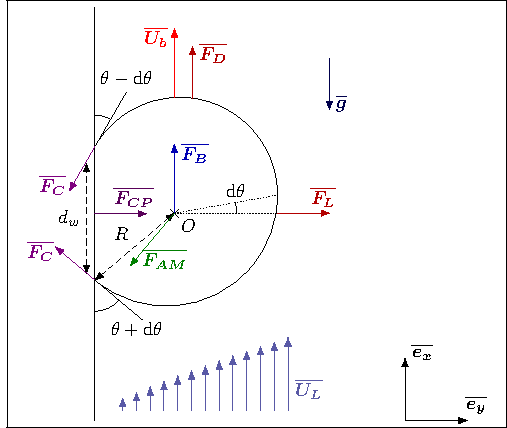
\includegraphics[width=0.6\linewidth]{img/forces/bub_bdf.pdf}
\caption{Sketch of the forces applied to the bubble facing an upward flow $\vect{U_{L}}$ and sliding at velocity $\vect{U_{b}}$}
\label{fig:bub_forces}
\end{figure}




Regarding the bubble shape, we consider a quasi-spherical bubble of radius $R$ with a circular contact area with the wall of radius $r_{w}$. It has a static contact angle $\theta$ and is tilted under the influence of the flow by an inclination angle $\dtheta$ (half the total angle hysteresis). The resulting downstream and upstream contact angles are therefore $\theta_{d}=\theta-\dtheta$ and $\theta_{u}=\theta+\dtheta$. If the bubble has a shape close to a truncated sphere, we can approximate the bubble foot radius as:

\begin{equation}
%r_{w}\approx \frac{1}{2} R~\parth{\sin{\theta_{u}} + \sin{\theta_{d}} }=R~\sin{\theta}\cos{\dtheta}
r_{w} \approx R~ \sin{\frac{\theta_{u}+\theta_{d}}{2}}=R~ \sin{\theta}
\label{eq:rw}
\end{equation}

We suppose $V_{b}\approx\frac{4}{3}\pi R^{3}$ for the bubble volume.

\subsection{Buoyancy Force}

The Buoyancy force results from both the weight of the bubble and the integration of the static liquid pressure over its surface which naturally yields:
\begin{equation}
\label{eq:buoyancy}
\vect{F_{B}}=V_{b}\parth{\rho_{V}-\rho_{L}}\vect{g}=\frac{4}{3}\pi R^{3}\parth{\rho_{L}-\rho_{V}}g \ \vect{e_{x}}
\end{equation}

\subsection{Capillary Force}\label{subsec:FC}

The most common and generally accepted expression of the capillary force has been derived by Klausner \cite{klausner_vapor_1993} by integrating the tangential effort at the triple contact line over the bubble foot radius while assuming an evolution of the contact angle from $\theta_{d}$ to $\theta_{u}$ as a polynomial expression of degree 3. This results in:

\begin{align}
\nonumber \vect{F_{C}}=&-\pi R \sigma \crocht{2.5~ \frac{r_{w}}{R} \frac{\dtheta}{\parth{\frac{\pi}{2}}^{2}-\dtheta^{2}}\sin{\theta}\cos{\dtheta}} \vect{e_{x}}\\
%
& - \pi R \sigma \crocht{2\ \frac{r_{w}}{R} \sin{\theta} \frac{\sin{\dtheta}}{\dtheta}}\vect{e_{y}}
\label{eq:FC_klausner}
\end{align}
%where $\sigma$ is the surface tension and $\displaystyle r_{w}\approx R\  \frac{\sin{\theta_{u}}+\sin{\theta_{d}}}{2}=R\ \sin{\theta}\cos{\dtheta}$.
%&\int_{0}^{2\pi} r_{w} \sigma \vect{\tau} \mathrm{d}\alpha\\
%=& -1.25\ \frac{2\pi r_{w}\sigma \parth{\theta_{u} - \theta_{d}} }{\pi^{2} - \parth{\theta_{u} - \theta_{d}}^{2} }\crocht{\sin{\theta_{u}} + \sin{\theta_{d}}}\ \vect{e_{x}} +\frac{2\pi r_{w} \sigma}{\theta_{u} - \theta_{d}}\crocht{\cos{\theta_{u}} - \cos{\theta_{d}}}\ \vect{e_{y}}\\


\subsection{Contact Pressure Force}\label{subsec:FCP}

The Contact Pressure force is linked to the overpressure inside the bubble. Combined with the Archimedes force, it can be expressed versus the difference of liquid and vapor pressure at the bubble foot using Laplace's equation as:
\begin{align}
\vect{F_{CP}}  \approx \frac{2\sigma}{R_{c}} \pi r_{w}^{2}\  \vect{e_{y}}
\approx \pi R \sigma\ 2\ \sin{\theta}^{2}\ \vect{e_{y}}
\label{eq:FCP}
\end{align}

Here, $R_{c}$ is the curvature radius of the bubble which is often assumed to be equal to $5R$ \cite{klausner_vapor_1993, sugrue_modified_2016, mazzocco_reassessed_2018} without other explanation than avoiding an overestimation of the Contact Pressure force. To avoid this arbitrary choice, following the hypothesis of a nearly spherical bubble shape gives $R_{c}=R$.
% apart that it helps the model to fit experimental measurements by ponderating the magnitude of the contact pressure force.

\subsection{Drag and Lift Forces}\label{subsec:FD}

The external liquid flow over the bubble induces the well-known Drag and Lift forces, acting respectively in the flow direction and perpendicular to the flow. They are usually expressed using associated coefficients $C_{D}$ and $C_{L}$ defined by:
\begin{align}
\vect{F_{D}}=&\frac{1}{2}C_{D}\rho_{L}S_{p} \norm{ \vect{U_{L}}-\vect{U_{b}} } \parth{\vect{U_{L}}-\vect{U_{b}}} \\
\vect{F_{L}}=&\frac{1}{2}C_{L}\rho_{L}S_{p}\norm{\vect{U_{L}}-\vect{U_{b}}}^{2}\ \vect{e_{y}}
\end{align}
with $S_{p}=\pi R^{2}$ the projected area of the bubble in the direction of the flow.


Traditional approaches rely on expressions of the Drag force for a bubble in an infinite medium based on numerical correlations as proposed by Mei \cite{mei_unsteady_1992}: 

\begin{equation}
C_{D,U} = \frac{16}{\Re_{b}}\crocht{1 + \parth{\frac{8}{\Re_{b}}+ \frac{1}{2}\parth{1+\frac{3.315}{\sqrt{\Re_{b}}} }}^{-1} }
\label{eq:CD_mei}
\end{equation}


Results from DNS conducted by Eames \etal \cite{eames_lift_2008} proposed expressions of the Drag and Lift forces for a hemispherical bubble on a wall facing a viscous shear flow. Earlier, Legendre \& Magnaudet \cite{legendre_lift_1998} analytically derived coefficients to transpose Drag and Lift expressions for a particle to the case of a bubble. This was applied by Mazzocco \etal \cite{mazzocco_reassessed_2018} to the Drag for a solid particle near a wall in a shear flow proposed by Zeng \etal \cite{zeng_forces_2009}.

In this work, we propose to rely on the recent work of Shi \etal \cite{shi_drag_2021} who conducted DNS of a shear flow over a spherical bubble of constant radius close to a wall for bubble Reynolds number between $10^{-1}$ and $10^{3}$ and shear rates between -0.5 and 0.5.

They computed the resulting Drag and Lift coefficients for each simulations and proposed correlations fitting their numerical results. The total Drag coefficient is expressed as a correction of the Drag coefficient for a bubble in an unbounded uniform flow  $C_{D,U}$. The total drag is given by:

\begin{equation}
C_{D}=\parth{1+\Delta C_{D}}C_{D,U}
\end{equation}
where $\Delta C_{D}$ accounts for both the effect of the shear flow and the wall vicinity. 

To cover the whole range of bubble Reynolds numbers, correlations at low and high $\Re_{b}$ are smoothly connected using an exponential term.

\begin{equation}
\Delta C_{D}=\Delta C_{D,\Re_{b}=O\parth{1}}+\parth{1-e^{-0.07\Re_{b}}}\Delta C_{D,{\Re_{b}\gg 1}}
\label{eq:drag_corr_shi}
\end{equation}


Each of those corrections is computed depending on $\Re_{b}$,  the non-dimensional shear rate $\Sr$, the non dimensional distances $L_{R} = \frac{y}{R}$ and $L_{u}= y \frac{\bars{U_{rel}}}{\nu_{L}}$  ($L_{R}=1$ being a spherical bubble laying on a wall). 


\begin{align}
\nonumber \Delta C_{D,\Re_{b}=O\parth{1}} = & \frac{1+\mathrm{tanh}\parth{0.012\Re_{b}^{0.8}} + \mathrm{tanh}\parth{0.07\Re_{b}^{0.8}}^{2}}{1+0.16L_{u}\parth{L_{u}+4}}
 \\
%
\nonumber &\times \left[ \left(\frac{3}{8}L_{R}^{-1} + \frac{3}{64}L_{R}^{-4}\right) \left(1- \frac{3}{8}L_{R}^{-1}-\frac{3}{64}L_{R}^{-4}\right)^{-1} \right.\\
&\left. \quad - \frac{1}{16}\left(L_{R}^{-2}+\frac{3}{8}L_{R}^{-3}\right)\text{Sr} \right]
\end{align}



\begin{align}
\nonumber \Delta C_{D,{\Re_{b}\gg 1}} =& ~0.47L_{R}^{-4}+0.0055L_{R}^{-6}\Re_{b}^{3/4} 
+0.002 \bars{\mathrm{Sr}}^{1.9} \Re_{b} \\
%
&+ 0.05 L_{R}^{-7/2} \mathrm{Sr} \Re_{b}^{1/3}
\end{align}


Figure \ref{fig:CD_shi} shows the evolution of the Drag correction $\Delta C_{D}$ against the bubble Reynolds number for different distances to the wall $L_{R}$ and two values of $\Sr$.  We can see that as the distance between the wall and the bubble increases the Drag correction logically approaches zero and that increasing the shear rate $\Sr$ increases $\Delta C_{D}$ for higher values of $\Re_{b}$.


Shi \etal \cite{shi_drag_2021} conducted DNS for wall distances down to $L_{R}=1.5$. However, Scheiff \etal \cite{scheiff_experimental_2021} compared the values obtained for $L_{R}=1$  with measured Drag coefficients of bubbles sliding on a wall and observed a good agreement, which legitimates the use of this new Drag correlation by extending its application to the case of a bubble laying on a wall and using the uniform drag coefficient of Eq.~\ref{eq:CD_mei}.




\begin{figure}[h!]
\centering
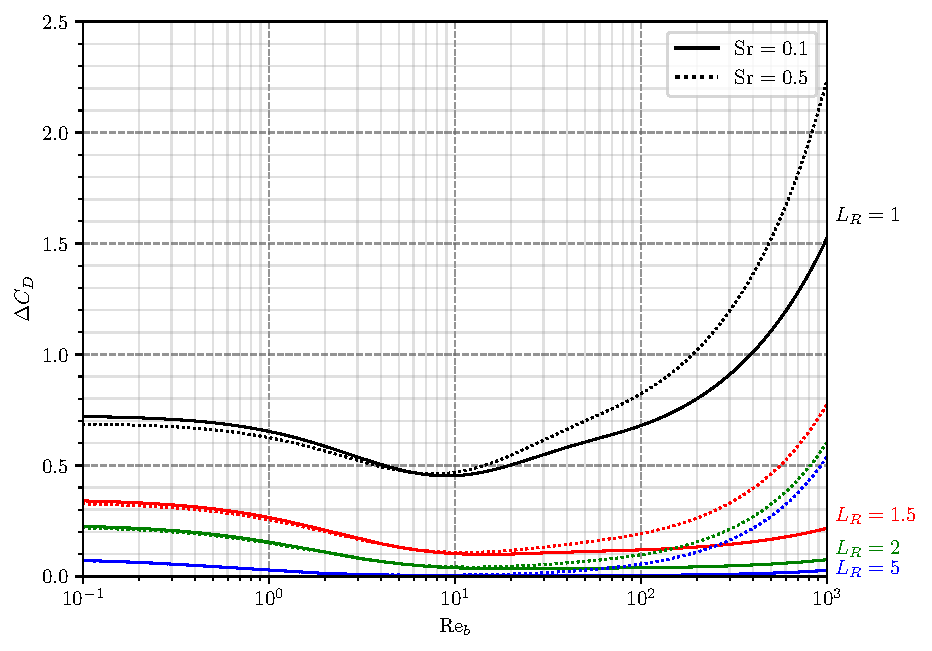
\includegraphics[width=0.8\linewidth]{img/forces/corr_drag.pdf}
\caption{Drag correction from Shi \etal \cite{shi_drag_2021}.}
\label{fig:CD_shi}
\end{figure}


\npar

Since this work focuses on the sliding, the total force balance will be studied along the $x$ axis, parallel to the wall. Thus, we do not detail the whole expression of Shi \etal for $C_{L}$. For further work, it is though interesting to mention that their expression of $C_{L}$ is based on the sum of three contributions (wall presence, shear and a coupled term) and changes sign when reaching negative values or $\Sr$ for instance.





\subsection{Inertia Force}
\label{subsec:AM}

The Inertia force originates from various effects (bubble growth, freestream and bubble acceleration, etc.) that includes both Added Mass and Tchen forces and is expressed as \cite{magnaudet_motion_2000}:

\begin{equation}
\vect{F_{I}} = \underbrace{ \rho_{L}V_{b}\parth{\dtime{\vect{U_{L}}}+\vecgrad{U_{L}}\cdot \vect{U_{L}}} }_{\text{Liquid inertia or Tchen force}} + \underbrace{ \derive{}{t}\parth{\rho_{L}C_{AM}V_{b}\parth{\vect{U_{L}}-\vect{U_{b}}}} }_{\text{Added Mass force } \vect{F_{AM}}}
\label{eq:F_inertia}
\end{equation}

Since we consider a steady and quasi-parallel liquid flow, the inertia term is equal to zero.



\subsubsection{Former Approaches}
\label{subsubsec:former_AM}

In previous Mechanistic Models, the derivation of the Added Mass force was conducted with different approaches. In particular, some authors have chosen to rely on the Rayleigh-Plesset Equation for a growing hemispherical bubble in a quiescent flow to obtain the reaction force from the liquid, oriented perpendicularly to the wall.

\begin{equation}
\vect{F_{AM,RPE}}=- \rho_{L}\pi R^{2}\crocht{R\ddot{R}+\frac{3}{2}\dot{R}^{2}}\vect{e_{y}}
\end{equation}

Then, assuming a bubble inclination angle $\theta_{i}$, this force is projected along the $x$ axis to obtain an Added Mass force parallel to the wall that hinders departure. The inclination angle value is often empiricial and used for data fitting \cite{zeng_unified_1993-1, colombo_prediction_2015, mazzocco_reassessed_2018, ren_development_2020}.

\begin{equation}
\vect{F_{AM,RPE}}=- \rho_{L}\pi R^{2}\crocht{R\ddot{R}+\frac{3}{2}\dot{R}^{2}}\parth{\sin{\theta_{i}}\vect{e_{x}} + \cos{\theta_{i}}\vect{e_{y}}}
\label{eq:AM_RPE}
\end{equation}


This approach is questionable on different aspects. First, the RPE assumes a moving boundary in a quiescent unbounded liquid, which is physically far from the real situation of a bubble growing on a wall in a boiling flow. Moreover, the subsequent projection along the different directions regarding an unknown angle is hardly reasonable if $\theta_{i}$ is chosen arbitrarily.



On the other hand, some authors \cite{klausner_vapor_1993, thorncroft_bubble_2001, guan_bubble_2015} considered two distinct contributions: 

\begin{itemize}

\item Hemispherical bubble growth in a stagnant liquid, leading to Eq.~\ref{eq:AM_RPE} including the inclination angle $\theta_{i}$ ;
\item Spherical bubble growth in an uniform unbounded and inviscid liquid flow, which yields a detaching Added Mass term  due to the interaction of bubble growth with the external flow: 
\begin{equation}
\vect{F_{AM,U}}= \frac{3}{2}\rho_{L}V_{b}\frac{\dot{R}}{R}U_{L} \vect{e_{x}} 
\label{eq:AM_bulk}
\end{equation} 

\end{itemize}

By including the effect of the liquid flow, this approach can be considered as closer to the reality. However, it relies on two separate derivations associated to different physical considerations.

\subsubsection{Proposed Approach}
\label{subsubsec:new_AM}

To tackle the Added Mass derivation in a proper way, we propose to follow the approach of Lamb \cite{lamb_hydrodynamics_1895} (also presented by Milne Thomson \cite{milne-thomson_theoretical_1938} or Van Winjgaarden \cite{wijngaarden_hydrodynamic_1976}). By solving the potential flow around a bubble and its image, we can obtain the total liquid kinetic energy $E_{L}$ that corresponds to a situation where a bubble is at a given distance from a wall (represented by the line normal to the line of centers of the bubbles). 

Then, using Lagrange's equations to compute the resulting forces in each direction:


\begin{align}
\label{eq:Lag_x}
F_{AM,x}&=-\dpartial{}{t}\parth{\dpartial{E_{L}}{\dot{x}}}+\dpartial{E_{L}}{x}\\
\label{eq:Lag_y}
F_{AM,y}&=-\dpartial{}{t}\parth{\dpartial{E_{L}}{\dot{y}}}+\dpartial{E_{L}}{y}
\end{align}


To express the liquid kinetic energy, we can rely on the work of Van Der Geld \cite{van_der_geld_dynamics_2009} who derived $E_{L}$ in the case of a full or truncated spherical bubble laying on a wall and facing an uniform flow parallel to the wall of velocity $U_{L}$ (Eq.~\ref{eq:EL_VdG}). If the bubble slides at a velocity $U_{b}=\dot{x}$, it sees a liquid velocity $U_{rel}=U_{L}-\dot{x}$.

\begin{align}
E_{L}=\frac{\rho_{L}V_{b}}{2}\parth{\alpha \dot{y}^{2} +\trb\dot{R}^{2}+\psi \dot{R}\dot{y} +\alpha_{2} \parth{U_{L}-\dot{x}}^{2} }
\label{eq:EL_VdG}
\end{align}
where $(x,y)$ are the coordinates of the bubble's center and $\alpha$, $\trb$, $\psi$, $\alpha_{2}$ are polynomials of $R/y = 1/L_{R}$ derived by Van Der Geld for $1<R/y<2$ \ie $0.5<L_{R}<1$.



Injecting $E_{L}$ in Eq.~\ref{eq:Lag_x} and \ref{eq:Lag_y} and computing the values for the sphere case ($y=R$ and $\dot{y} = \dot{R}$) yields:

\begin{align}
F_{AM,x}=\rho_{L}V_{b}\crocht{3C_{AM,x}\frac{\dot{R}}{R}U_{rel} - C_{AM,x}\dtime{U_{b}}}
\label{eq:AMx}
\end{align}
with $C_{AM,x} \approx 0.636$.


\begin{align}
F_{AM,y}=\rho_{L}V_{b}\crocht{-\parth{3 C_{AM,y1} + C_{AM,y2}}\frac{\dot{R}^{2}}{R}-C_{AM,y1}\ddot{R} + C_{AM,y3}\frac{U_{rel}^{2}}{R}}
\label{eq:AMy}
\end{align}
with $C_{AM,y1} \approx 0.27$, $C_{AM,y2}\approx 0.326$ and $C_{AM,y3}\approx 8.77\times  10^{-3}$.


\npar
 
 


Parallel to the wall, the coupled term $\frac{\dot{R}}{R}U_{rel}$ in Eq.~\ref{eq:AMx} promotes detachment and sliding of the bubble if $U_{rel}>0$ \eg if the bubble is attached to its nucleation site. This relatively agrees with the detaching term of the "two situations" derivations detailed in \ref{subsubsec:former_AM} and clearly contradicts the aforementioned approach where solely projecting the RPE on both axes lead to an Added-Mass term related to bubble growth that only hinders the departure by sliding. 

Moreover, Eq.~\ref{eq:AMy} exhibits a term induced by the relative velocity that acts as a lift force, which seems to rarely appear in other approaches.

\npar
Here we want to insist on the importance on conducting an approach as rigorous as possible when deriving those transient aspects of the force balance. Otherwise, some terms may be missing and lead to contradictory physical conclusions. Although the proposed method has already been used in different works, we obtained revisited values of the Added Mass coefficients based on the derivation of the liquid kinetic energy by Van Der Geld.

In the spirit of avoiding to introduce extra empirical terms, we keep the Added Mass force as presented in Eq.~\ref{eq:AMx} and \ref{eq:AMy}. No projection of the $y$ term along the $x$ axis to account for asymmetric bubble growth is considered in this study.


\subsection{Force Balance Summary}\label{subsec:BdF}


On Table \ref{tab:all_BdF}, we sum up some of the mentioned force balance approaches and their models.



\begin{table}[H]



\scriptsize
\centering

\noindent\makebox[\textwidth]{
\renewcommand{\arraystretch}{2.0}


\begin{tabular}{p{2mm} p{6mm}|p{50mm}|p{50mm}|p{50mm}}

 & & Klausner (1993) \cite{klausner_vapor_1993} & Thorncroft (2001) \cite{thorncroft_bubble_2001} & Sugrue (2016) \cite{sugrue_modified_2016} \\
\hline

\multirow{6}*{\rotatebox{90}{Forces}} &  $\vect{F_{B}}$ & $\frac{4}{3}\pi R^{3} \parth{\rho_{L}-\rho_{V}}\vect{g}$ & $\frac{4}{3}\pi R^{3}\parth{\rho_{L}-\rho_{V}}\vect{g}$ & $\frac{4}{3}\pi R^{3}\parth{\rho_{L}-\rho_{V}}\vect{g}$ \\

& $\vect{F_{C}}$ & Eq. \ref{eq:FC_klausner}, $r_{w}=0.045$ mm & Eq. \ref{eq:FC_klausner}, $r_{w}=R~\sin{\theta_{d}}$ & Eq. \ref{eq:FC_klausner}, $r_{w}=0.025R$ \\

& $\vect{F_{CP}}$ &  Eq.~\ref{eq:FCP}, $R_{c}=5R$ &  Neglected &  Eq.~\ref{eq:FCP}, $R_{c}=5R$  \\

& \multirow{2}*{$\vect{F_{D}}$} & $C_{D}=\frac{16}{\Re_{b}} \left[ 1+\frac{3}{2} \left( \parth{\frac{12}{\Re_{b}}}^{n}\right. \right.$\newline$ \left. \left. \quad \quad + 0.796^{n} \right) ^{1/n} \right]$, $n=0.65$ & $C_{D} = \frac{16}{\Re_{b}} \left[ 1 + \left(\frac{8}{\Re_{b}} \right. \right.$\newline$\left. \left. \quad  \quad + \frac{1}{2}\parth{1+\frac{3.315}{\sqrt{\Re_{b}}} } \right)^{-1} \right]$ & $C_{D}=\frac{16}{\Re_{b}} \left[ 1+\frac{3}{2} \left( \parth{\frac{12}{\Re_{b}}}^{n}\right. \right.$\newline$ \left. \left. \quad \quad + 0.796^{n} \right) ^{1/n} \right]$, $n=0.65$ \\

& \multirow{2}*{$\vect{F_{L}}$} & $C_{L}=2.74\sqrt{\Sr}$\newline$\times\crocht{\Re_{b}^{-2} + \parth{0.24\sqrt{\Sr}}^{4} }^{\frac{1}{4}}$ & $C_{L}=0.71\sqrt{\Sr}$\newline$\times\crocht{\parth{\frac{1.15\mathrm{J}(\varepsilon)}{\sqrt{\Re_{b}}}}^{2} + \parth{\frac{3\sqrt{2\Sr}}{8}}^{2} }^{\frac{1}{2}}$ & $C_{L}=2.74\sqrt{\Sr}$\newline$\times\crocht{\Re_{b}^{-2} + \parth{0.24\sqrt{\Sr}}^{4} }^{\frac{1}{4}}$   \\

& \multirow{2}*{$\vect{F_{AM}}$} & {$\frac{3}{2}\rho_{L}V_{b}\frac{\dot{R}}{R}U_{L} \vect{e_{x}}$ {$-\rho_{L}\pi R^{2}\parth{\frac{3}{2}\dot{R}^{2} + R\ddot{R}}$\newline$\times \parth{\cos{\theta_{i}}\vect{e_{y}} + \sin{\theta_{i}}\vect{e_{x}}}$, $\theta_{i}=10\degree$ }} & {$2\pi \rho_{L}R^{2}\dot{R}U_{L}\vect{e_{x}}$} {$-\rho_{L}\pi R^{2}\parth{\frac{3}{2}\dot{R}^{2} + R\ddot{R}}$\newline$\times \parth{\cos{\theta_{i}}\vect{e_{y}} + \sin{\theta_{i}}\vect{e_{x}}}$, $\theta_{i}=45\degree$ } & {{$-\rho_{L}\pi R^{2}\parth{\frac{3}{2}\dot{R}^{2} + R\ddot{R}}$\newline$\times \parth{\cos{\theta_{i}}\vect{e_{y}} + \sin{\theta_{i}}\vect{e_{x}}}$, $\theta_{i}=10\degree$ }} \\
\hline
\end{tabular}
}

\npar

\noindent\makebox[\textwidth]{
\renewcommand{\arraystretch}{2.0}

\begin{tabular}{p{2mm} p{6mm}|p{50mm}|p{50mm}|p{50mm}}
 & & Mazzocco (2018) \cite{mazzocco_reassessed_2018} & Ren (2020) \cite{ren_development_2020} & Present model \\
\hline

\multirow{6}*{\rotatebox{90}{Forces}} &  $\vect{F_{B}}$ & $\frac{4}{3}\pi R^{3} \parth{\rho_{L}-\rho_{V}}\vect{g}$ & $\frac{4}{3}\pi R^{3} \parth{\rho_{L}-\rho_{V}}\vect{g}$ & $\frac{4}{3}\pi R^{3} \parth{\rho_{L}-\rho_{V}}\vect{g}$ \\

& $\vect{F_{C}}$ & Eq. \ref{eq:FC_klausner}, $r_{w}=R/15$ & Eq. \ref{eq:FC_klausner}, $r_{w}=0.2R$& Eq. \ref{eq:FC_klausner}, $r_{w}=R\ \sin{\theta}$ \\

& $\vect{F_{CP}}$ & Eq.~\ref{eq:FCP}, $R_{c}=5R$ &  Eq.~\ref{eq:FCP}, $R_{c}=5R$ &  Eq.~\ref{eq:FCP}, $R_{c}=R$   \\

& \multirow{2}*{$\vect{F_{D}}$} & \multirow{2}*{$C_{D}=1.13\frac{24}{\Re_{b}}\parth{1+0.104\Re_{b}^{0.753}}$} & $C_{D}=\frac{16}{\Re_{b}} \left[ 1+\frac{3}{2} \left( \parth{\frac{12}{\Re_{b}}}^{n}\right. \right.$\newline$ \left. \left. \quad \quad + 0.796^{n} \right) ^{1/n} \right]$, $n=0.65$ & $C_{D}=C_{D,U}\parth{1+\Delta C_{D}}$ \newline $C_{D,U}$ by Eq. \ref{eq:CD_mei}, $\Delta C_{D}$ by Eq. \ref{eq:drag_corr_shi} \\

& \multirow{2}*{$\vect{F_{L}}$} & \multirow{2}*{$C_{L}=2.61$} & $C_{L}=2.74\sqrt{\Sr}$\newline$\times\crocht{\Re_{b}^{-2} + \parth{0.24\sqrt{\Sr}}^{4} }^{\frac{1}{4}}$ & \multirow{2}*{$C_{L}$ by Shi \etal \cite{shi_drag_2021}}   \\

& \multirow{2}*{$\vect{F_{AM}}$} & {$-\frac{1}{4}\pi \rho_{L} K^{4}\parth{\cos{\theta_{i}}\vect{e_{y}} + \sin{\theta_{i}}\vect{e_{x}}}$, $\sin{\theta_{i}}=0.2$, $\cos{\theta_{i}}=1$} & {$-\rho_{L}\pi R^{2}\parth{\frac{3}{2}\dot{R}^{2} + R\ddot{R}}$\newline$\times \parth{\cos{\theta_{i}}\vect{e_{y}} + \sin{\theta_{i}}\vect{e_{x}}}$, $\theta_{i}=15\degree$ } & {$\frac{F_{AM,x}}{\rho_{L}V_{b}}=C_{AM,x}\crocht{3\frac{\dot{R}}{R}U_{rel} - \dtime{U_{b}}}$, $C_{AM,x}=0.636$, $F_{AM,y}$ by Eq. \ref{eq:AMy}.} \\
\hline
\end{tabular}

}


\caption{Summary of different force-balance mechanistic approaches.}
\label{tab:all_BdF}
\end{table}


\subsection{Liquid Velocity}\label{subsec:liq_vel}

To compute the liquid velocity and shear rate at bubble center height, we use the wall law of Reichardt \cite{reichardt_vollstandige_1951}, which describes the velocity profile from the viscous sublayer to the logarithmic region.

\begin{align}
U_{L}^{+} =& \frac{1}{\kappa}\ln{1+\kappa y^{+}} + c \parth{1-e^{-y^{+}/\chi} + \frac{y^{+}}{\chi}e^{-y^{+}/3} }\\
%
\nonumber U_{L}=&U_{L}^{+}U_{\tau}
\end{align}
with $\kappa = 0.41$, $\chi = 11$ and $c=7.8$.

\begin{align}
\dpartial{U_{L}^{+}}{y^{+}} =& \frac{1}{1+\kappa y^{+}}+\frac{c}{\chi}\parth{e^{-y^{+}/\chi} + \parth{1-\frac{y^{+}}{3}}e^{-y^{+}/3}}\\
%
\nonumber \dpartial{U_{L}}{y} =& \gamma = \frac{U_{\tau}^{2}}{\nu_{L}} \dpartial{U_{L}^{+}}{y^{+}}
\end{align}

The friction velocity is computed using Mac Adams correlation \cite{mcadams_heat_1954}.

\begin{align}
U_{\tau} =& \sqrt{\frac{\tau_{w}}{\nu_{L}}}\\
\tau_{w} =& 0.018~ \Re_{D_{h}}^{-0.182}~ \frac{G_{L}^{2}}{\rho_{L}}
\end{align}

\section{Departure by Sliding}\label{sec:departure}

\subsection{Non-Dimensional Analysis}\label{subsec:adim_dep}

Now that the force balance has been established, we can write it parallel to the wall before bubble departure by sliding \ie $U_{b}=\dtime{U_{b}}=0$.

\begin{align}
\label{eq:sum_dep}
\nonumber - \pi R\sigma f_{C,x} + \frac{4}{3}\pi R^{3}\parth{\rho_{L}-\rho_{V}}g &+ \frac{1}{2}C_{D}\rho_{L}\pi R^{2} U_{L}^{2} \\
& + \frac{4}{3}\pi R^{3}\rho_{L}~3C_{AM,x}\frac{\dot{R}}{R}U_{L} = 0
\end{align}

\begin{equation}
 f_{C,x}=2.5\ \frac{\dtheta}{\parth{\pi/2}^{2}-\dtheta^{2}}\sin{\theta}^{2}\cos{\dtheta}
\end{equation}
with $f_{C,x} \to 0 $ if $\dtheta \to 0$.


We can note that the departure by sliding is promoted by the Buoyancy, the Drag and the Added Mass forces. Only the Capillary force keeps the bubble attached to its nucleation site, which will be discussed later.


\npar
Re-writing Eq.~\ref{eq:sum_dep} in non-dimensional form by dividing the LHS by the Added Mass force yields:

\begin{equation}
\label{eq:adim_dep}
-\frac{1}{2}\frac{f_{C,x}}{K^{2}C_{AM,x}}\frac{1}{\Ca}\frac{\Pr_{L}}{\Ja_{w}^{2}} +  \frac{1}{3}\frac{1}{K^{2}C_{AM,x}}\frac{\Re_{b}}{\Fr}\frac{\Pr_{L}}{\Ja_{w}^{2}} + \frac{1}{8}\frac{C_{D}}{K^{2}C_{AM,x}}\Re_{b}\frac{\Pr_{L}}{\Ja_{w}^{2}} +1 =0
\end{equation}
where we have the following non-dimensional numbers:
\begin{align}
\nonumber \Re_{b} =& \frac{2RU_{L}}{\nu_{L}}\ ;\ \Fr=\frac{\rho_{L}U_{L}^{2}}{\parth{\rho_{L}-\rho_{V}}g R}\ ;\ \We=\frac{\rho_{L}U_{L}^{2}R}{\sigma}\ ; \ \Eo=\frac{\parth{\rho_{L}-\rho_{V}}g R^{2}}{\sigma}\ ;\\
%
\nonumber \Ja_{w}=&\frac{\parth{T_{w}-T_{sat}}\rho_{L} c_{P,L}}{\rho_{V} h_{LV}}\ ;\ \Pr_{L}=\frac{\nu_{L}}{\eta_{L}}\ ;\ \frac{\dot{R}}{U_{L}}=\frac{K^{2}\Ja_{w}^{2}}{\Pr_{L} \Re_{b}}\ ;\ \Ca=\frac{\mu_{L}U_{L}}{\sigma}
\end{align}
%=\Re_{b}^{2}\frac{\rho_{L}\nu_{L}^{2} }{g\parth{\rho_{L}-\rho_{V}}4R^{3}} 


Eq.~\ref{eq:adim_dep} exhibits terms that can be used to compare the magnitude of each detaching forces. We can obtain the following conditions:

\begin{align}
&\text{Added Mass greater than Drag if:}\ \ \frac{\Ja_{w}^{2}}{\Pr_{L}}>\frac{1}{8}\frac{C_{D}}{C_{AM,x}}\frac{1}{K^{2}}\Re_{b} \label{eq:AMvsD}\\
&\text{Added Mass greater than Buoyancy if:}\ \  \frac{\Ja_{w}^{2}}{\Pr_{L}}>\frac{1}{3}\frac{1}{C_{AM,x}K^{2}}\frac{\Re_{b}}{\Fr} \label{eq:AMvsB}\\
&\text{Drag greater than Buoyancy if:}\ \  \Re_{b}>\frac{16}{3}\frac{1}{C_{D}}\frac{\Eo}{\Ca}=\Re_{c} \label{eq:DvsB}
\end{align}


Those boundaries can be plotted on a $\parth{\Ja_{w}^{2}/\Pr\ ;\ \Re_{b}}$ map for a given fluid and bubble diameter $D$. An example of such a map is presented on Figure \ref{fig:ND_map1}. This allows to visualize the operating conditions under which each of the detaching forces will be dominant. Logically, Buoyancy dominates for low $\Re_{b}$ regimes contrary to Drag. Added Mass dominates when values of $\Ja_{w}^{2}/\Pr_{L}$ are high \ie when bubble grows rapidly.





\begin{figure}[h!]
\centering
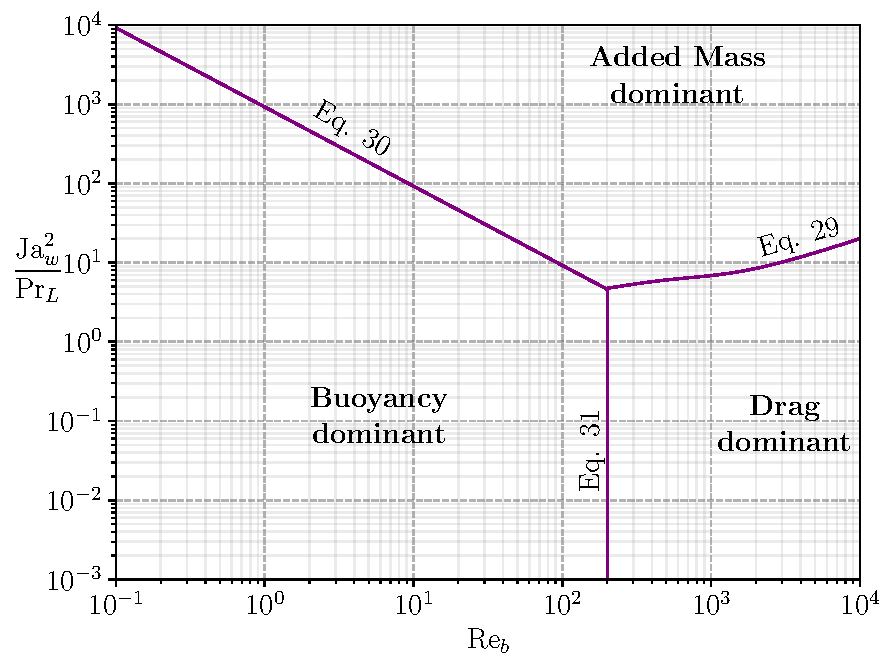
\includegraphics[width=0.7\linewidth]{img/forces/ND_map1.pdf}
\caption{Dominance map regarding departure by sliding. Boundaries plotted for water at 1 bar and $D_{d}=0.5$mm. ($K=2$)}
\label{fig:ND_map1}
\end{figure}



\subsubsection{Influence of Pressure}

On Figure \ref{fig:press_map}, we draw the dominance map for 3 different pressures and associated orders of magnitude of bubble departure diameter \cite{kocamustafaogullari_pressure_1983}.

The impact of pressure is mostly seen through the decrease of bubble departure diameter. As pressure increases, Buoyancy force decreases while Drag and Added Mass forces display much larger dominance zones. The competition between those two terms mainly relies on the competition between liquid flow velocity and wall superheat or heat flux.

 
\subsubsection{Comparison between Fluids}

 
On Figure \ref{fig:R12_PWR}, we compare the dominance zones for R12 at 26 bar and water at 155 bar. Moderately pressurized R12 (10 to 30 bar) has often been used as a simulating fluid to mimic water in PWR since it has the same density ratio and Weber number for instance.

Assuming that the conservation of Weber and Boiling numbers may lead to similar bubble departure diameters, we can observe that the boundaries between the two fluids are very close. This qualitatively indicates that R12 shall present bubble departure by sliding mechanisms similar to what happens in PWR, which could comfort the confidence one may have in extrapolating the observations done using the simulating fluid to industrial applications.






\begin{figure}[h!]
\centering
\subfloat[Dominance map plotted for water at different pressures and bubble departure diameters. ($K=2$)]{
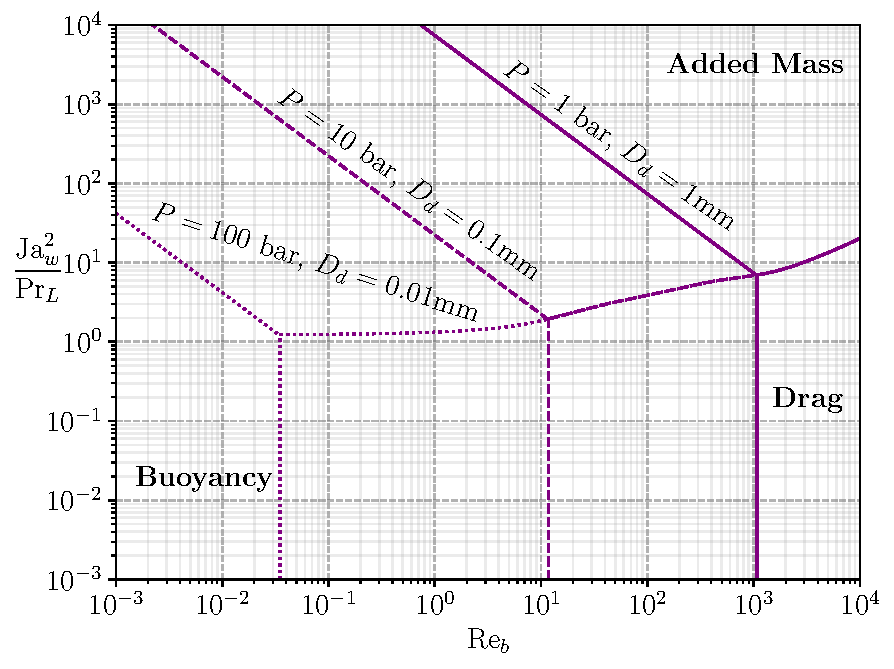
\includegraphics[width=0.7\linewidth]{img/forces/press_map.pdf}
\label{fig:press_map}
}
\\
\subfloat[Dominance map for R12 as simulating fluid for PWR. $D_{d}=0.05$mm is chosen according to R12 measurements from Garnier \etal \cite{garnier_local_2001} who observed bubbles of $\sim 0.1$mm diameter after lift-off. ($K=2$)]{
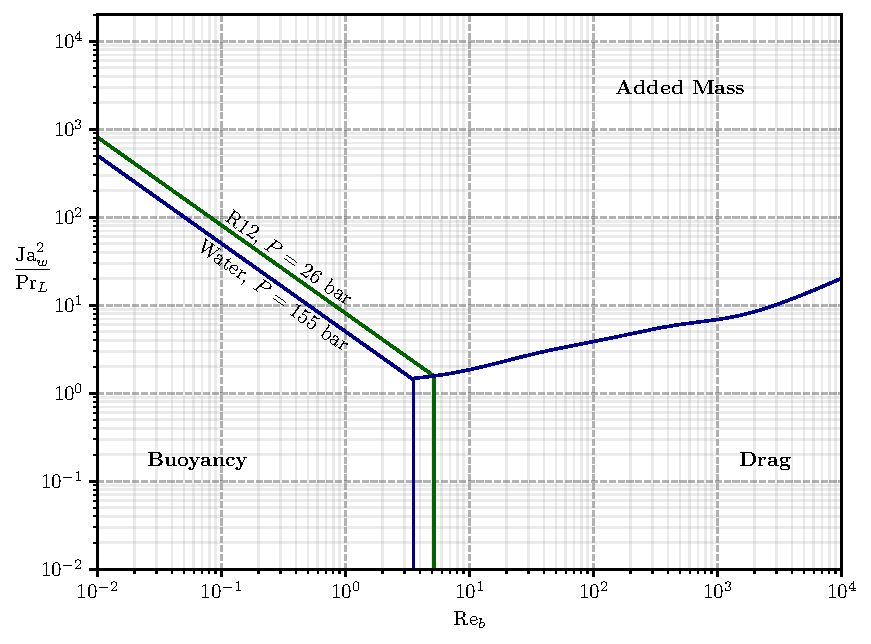
\includegraphics[width=0.7\linewidth]{img/forces/R12_PWR.pdf}
\label{fig:R12_PWR}
}
\caption{Examples of qualitative analysis using the non-dimensional regime map}
\end{figure}






\subsection{Application to Experimental Data}\label{subsec:data_map}

Now we want to apply this non-dimensional approach to experimental measurement in order to determine the actual bubble departure by sliding regimes. We rely on 7 experiments in which bubble departure diameters in vertical flow boiling were measured. The operating conditions are gathered in Table~\ref{tab:exp_data}.




\begin{table}[h!]

%\begin{changemargin}{-1cm}{0cm}
%\rowcolors{1}{}{lightbrown}
\noindent\makebox[\textwidth]{

\scriptsize
\centering
\begin{tabular}{p{20mm}|c c c c c c c c} 
Author & Fluid & $D_{h}$ [mm] & $P$ [bar] & $G_{L}$ [$\debm$] & $\Delta T_{L}$ [K] & $\phi_{w}$ [kW/m\up{2}] & $\Delta T_{w}$ [K] & $D_{d}$ [mm] ($N_{mes}$)\\
\hline
\\
Thorncroft \cite{thorncroft_experimental_1998} \newline (1998)& FC-87 & 12.7 & N.A. & 0 - 319 & 0.99 - 3.27 & 2.83 - 11.8 &  0.54 - 6.89 & 0.094 - 0.237  (10)\\
\\
Maity \cite{maity_effect_2000} \newline (2000) & Water & 20 & 1.01 & 0 - 239.6 & 0.3 - 0.7 & N.A. & 5 - 5.9 & 0.788 - 1.71 (9) \\
\\
Chen \cite{chen_prediction_2012} \newline (2012) & Water & 3.8 & 1.2 - 3.35 & 214 - 702 & 14.5 - 30.3 & 83.6 - 334 & N.A. & 0.549 - 2.255 (22)\\
\\
Sugrue \cite{sugrue_modified_2016} \newline (2014) & Water & 16.6 & 1.01 & 250 - 400 & 10 - 20 & 50 - 100 & 2 - 6 & 0.229 - 0.391 (16)\\
\\
Guan \cite{guan_bubble_2015} \newline (2014) & Water & 9 & 1.01 & 87.3 - 319.2 & 8.5 - 10.5 & 68.2 - 104 & 4.5 - 8.5 & 0.62 - 1.85 (12) \\
\\
Ren \cite{ren_development_2020} \newline (2020) & Water & 3.8 & 2 - 5.5 & 488.4 - 1654 & 28.7 - 51 & 160.7 - 643.2 &  N.A. & 0.045 - 0.111 (42) \\
\\
Kossolapov \cite{kossolapov_experimental_2021} \newline (2021) & Water & 11.8 & 19.9 - 39.8 & 500 - 1500 & 10 & 178 - 613 & N.A. & 0.01 - 0.047 (11) \\
\hline
\end{tabular}
}


\caption{Bubble departure diameters data sets in vertical flow boiling}
\label{tab:exp_data}

%\end{changemargin}

\end{table}





If the value of $\Delta T_{w}$ is not available in the considered data-set, we estimate it $\Delta T_{w}$ using Frost \& Dzakowic correlation \cite{frost_extension_1967}.

\begin{equation}
\Delta T_{w} = \Pr_{L,sat} \sqrt{\frac{8 \sigma \phi_{w} T_{sat}}{\lambda_{L}\rho_{V}h_{LV}}}
\label{eq:frost}
\end{equation}

Comparisons with bubble growth profile from Kossolapov \cite{kossolapov_experimental_2021} showed that values of $K$ respectively around $7$ and $15$ were needed to match experimental measurements at $20$ bar and $40$ bar. This means Eq.~\ref{eq:frost} probably underestimates the wall superheat on those cases. We will thus further adopt a corrective factor of $7$ at $20$ bar and $15$ at $40$ bar to use more realistic values of $K$.


\npar 

To place experimental measurements on the non-dimensional map, we need a bubble detachment diameter value $D_{d}$ to plot the dominance zones. Since measured $D_{d}$ vary significantly in each experiment, we draw the boundaries for the maximum and minimum values of $D_{d}$ as shown on Figure \ref{fig:exp_maity}. If the considered data covers different pressures, boundaries for each pressure are plotted to exhibit its impact (Figures \ref{fig:exp_chen}, \ref{fig:exp_ren} and \ref{fig:exp_koss}). We chose a value of $K=1$ to draw the boundaries.


The Figure \ref{fig:exp_maps} shows that for most of the low pressure experiments, the detaching forces are the Added Mass and the Buoyancy. Smaller bubbles are mainly detached under the effect of the Added Mass force (Figures \ref{fig:exp_sugrue}, \ref{fig:exp_chen} and \ref{fig:exp_ren}). When the bubbles detach at higher diameters, the impact of the Buoyancy force naturally increases and is comparable to the Added Mass force (Figures \ref{fig:exp_maity} and \ref{fig:exp_guan}).

When the pressure increases, we observe that the experimental measurements gradually move towards the Drag dominant zone as seen on Figures \ref{fig:exp_ren} and \ref{fig:exp_koss}. This main difference in the dynamic regime when bubble departs by sliding arises from multiple effects:

\begin{itemize}
\item The decrease of $\rho_{L}/\rho_{V}$ with pressure, thus reducing $\Ja_{w}$ and the impact of the detaching Added Mass term ;
\item The higher liquid mass fluxes in Kossolapov experiments, increasing the impact of the Drag ;
\item The decrease of $D_{d}$ with pressure, reducing the magnitude of Buoyancy.
\end{itemize}

However, we see that some measurements lie close to the Added Mass / Drag boundary (Figure \ref{fig:exp_koss}), indicating that the Added Mass force still plays a significant role for bubble detachment. This means that regardless of the operating pressure, the detaching term associated to the coupling between bubble growth and outer liquid flow should not be neglected in the force balance (Eq. \ref{eq:AMx}).




\begin{figure}[h!]
\begin{center}
\subfloat[Maity data]{
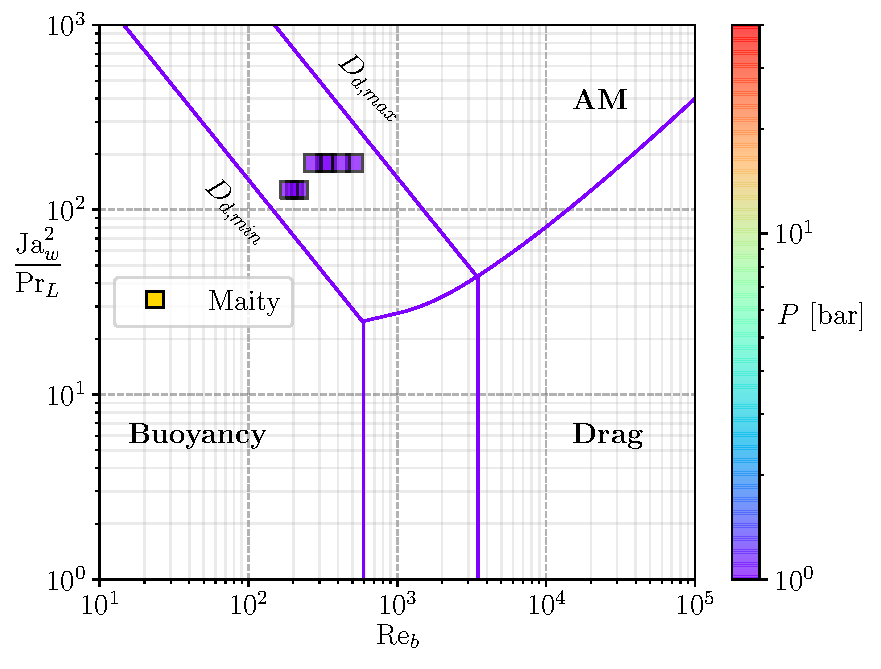
\includegraphics[width=0.45\linewidth]{img/forces/Maity_2.pdf}
\label{fig:exp_maity}
} 
\subfloat[Guan data]{
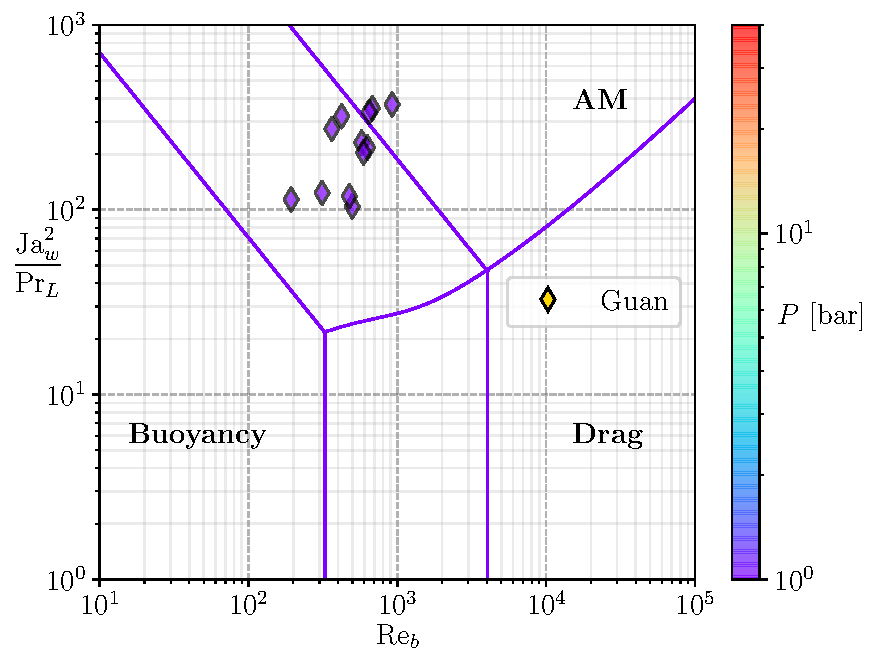
\includegraphics[width=0.45\linewidth]{img/forces/Guan_2.pdf}
\label{fig:exp_guan}
}
\\
\subfloat[Sugrue data]{
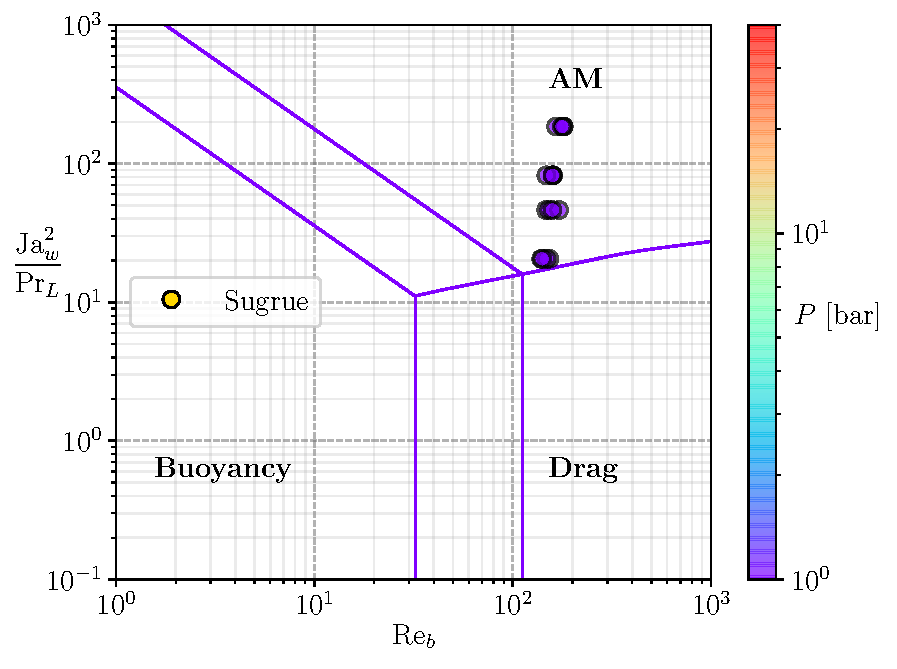
\includegraphics[width=0.45\linewidth]{img/forces/Sugrue_2.pdf}
\label{fig:exp_sugrue}
} 
\subfloat[Chen data]{
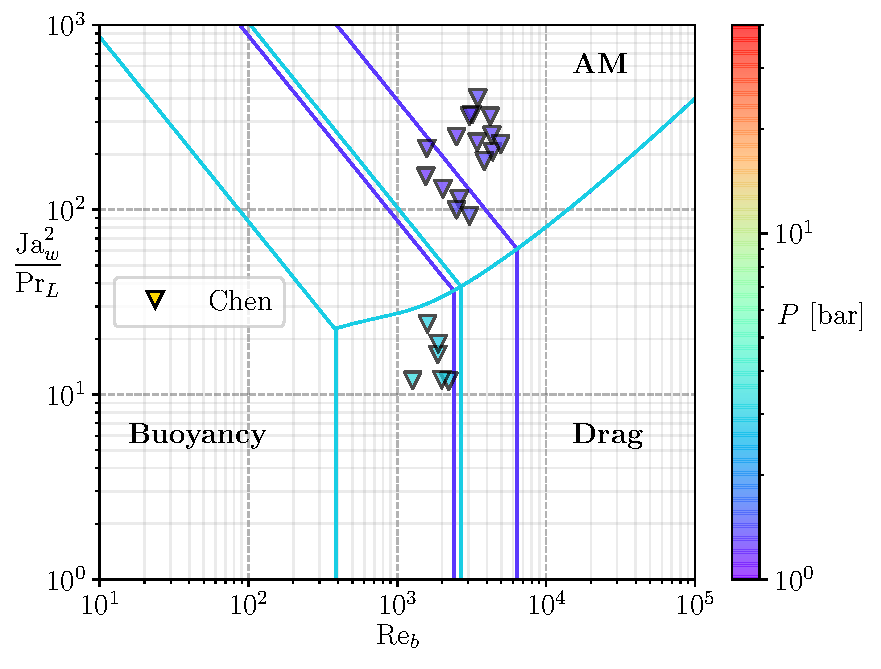
\includegraphics[width=0.45\linewidth]{img/forces/Chen_2.pdf}
\label{fig:exp_chen}
}
\\
\subfloat[Ren data]{
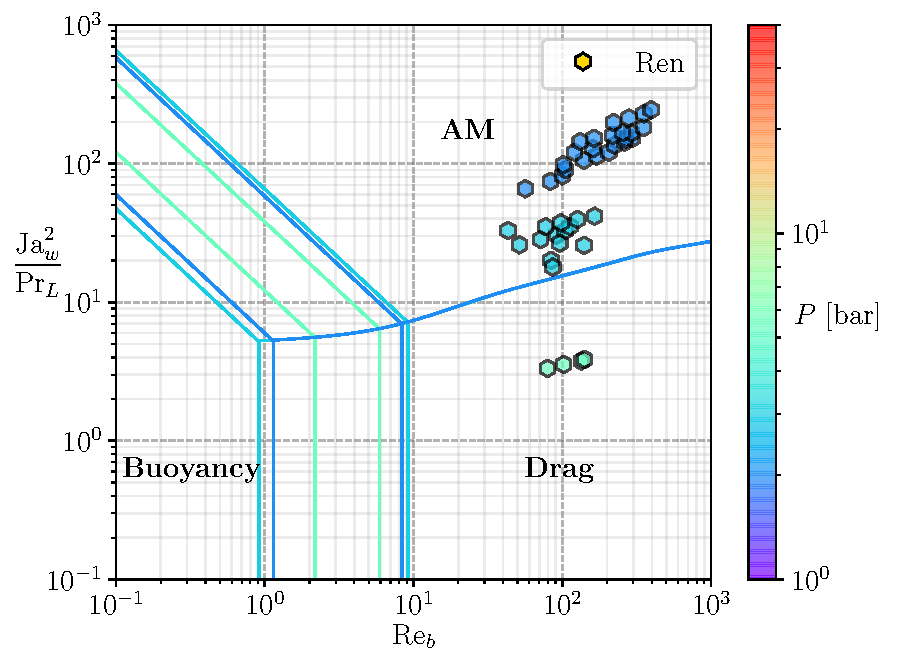
\includegraphics[width=0.45\linewidth]{img/forces/Ren_2.pdf}
\label{fig:exp_ren}
} 
\subfloat[Kossolapov data]{
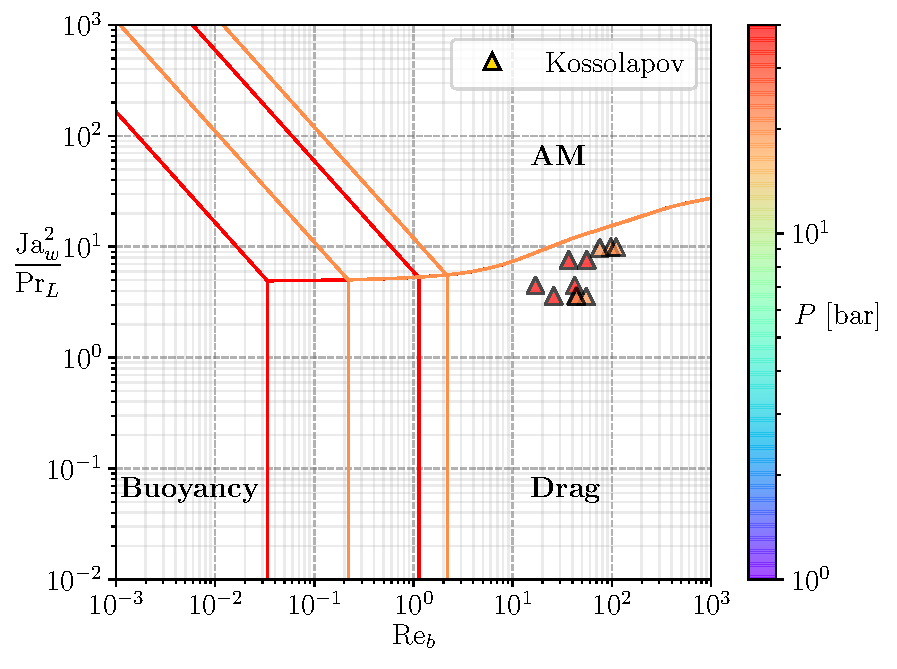
\includegraphics[width=0.45\linewidth]{img/forces/Kossolapov_2.pdf}
\label{fig:exp_koss}
}


	\caption{Dominance maps for each water data sets from Table \ref{tab:exp_data}.}	
	\label{fig:exp_maps}
\end{center}
\end{figure}



\subsection{Departure Diameter Prediction}\label{subsec:Dd_pred}

\subsubsection{About the Use of Empiricism}
 
As previously mentioned, the case of bubble detachment in vertical flow boiling is particular since only one force maintains the bubble attached to its nucleation site: the Capillary force (Eq.~\ref{eq:FC_klausner}). Its expression depends on the contact angle $\theta$, the angle half-hysteresis $\dtheta$ and the bubble foot radius $r_{w}$ (or ratio to bubble diameter $r_{w}/R$) and is thus very sensitive to those values. Paradoxically, those terms are among the least precisely known due to the difficulty of measurement and associated uncertainties. For instance, conducting precise evaluations of the contact angle near the bubble base through optical techniques can be challenging because of the strong temperature gradients close to the heated surface. 

Consequently, empirical choices have to be made in order to set a value to those parameters, often by relying on data-fitting or approximate measurements in other conditions. For instance, contact angles are often taken as arbitrary average values \cite{ren_development_2020} or measurements in room conditions \cite{sugrue_modified_2016} and applied over a whole set of experiments. This is questionable since contact angle is unlikely to remain unchanged over different operating conditions and surfaces with varying roughness and properties \cite{song_temperature_2021}.

However, no better information except those given by the authors can be used to evaluate the Capillary force since no generic model exist to compute the contact angle and hysteresis. In this work, admitting a significant uncertainty (typically $5\degree$, as in Guan \cite{guan_bubble_2015}), we will use the following values for the contact angles :


\begin{itemize}
\item $\theta_{u}=25.3\degree$ and $\theta_{d} = 6.6\degree$ for Thorncroft data (measured values for FC-87 on nichrome \cite{thorncroft_bubble_2001}) ;
\item $\theta_{u} = 50\degree$ and $\theta_{d} = 40\degree$ for Maity data (measured average contact angles for each bubble during its lifetime \cite{maity_effect_2000}) ;
\item $\theta_{u} = 130\degree$ and $\theta_{d} = 65\degree$ for Chen data (chosen values in their study following measurements for water on stainless steel at high temperature by Kandlikar \etal \cite{kandlikar_contact_2002}) ;
\item $\theta_{u}=91\degree$ and $\theta_{d} = 8\degree$ for Sugrue data (measured values at room temperature \cite{sugrue_effects_2012}) ;
\item $\theta_{u} = 75\degree$ and $\theta_{d} = 30\degree$ for Guan data (measured average value through experimental visualizations \cite{guan_bubble_2015}) ;
\item $\theta_{u} = 45\degree$ and $\theta_{d} = 36\degree$ for Ren data (chosen values in their study \cite{ren_development_2020}) ;
\item $\theta = 80 \degree$ for Kossolapov data (typical contact angle for water on ITO \cite{kossolapov_experimental_2021}) and $\dtheta=1\degree$ assuming that the very small bubbles at high pressure are nearly not tilted.
\end{itemize}


Similarly, the bubble foot radius $r_{w}$ is often empirically assumed to be either constant \cite{klausner_vapor_1993} proportional to the bubble radius \cite{sugrue_modified_2016, mazzocco_reassessed_2018} or to follow a linear or logarithmic law of $R$ \cite{zhou_experimental_2020, guan_bubble_2015}. That is why we chose to use the truncated sphere hypothesis (Eq. \ref{eq:rw}) to compute $r_{w}$ using $R$ and $\theta$.

Finally, we would like to acknowledge that the empiricism to evaluate those parameters represents one of the biggest flaws of the force-balance approach. Indeed, such a model aims to detect small sign changes in a sum of a few $\mu\mathrm{N}$ of forces that are decades larger as pointed out by Bucci \etal \cite{bucci_not-so-subtle_2021}. Mechanistic models are thus strongly sensitive to any extra parameter included in the modeling of the forces.

\subsubsection{Growth Constant Values}

Since the value $K\approx 2 $ represents an upper bound for the growth constant in a quiescent uniformly superheated liquid \cite{plesset_growth_1954} and that values below 1 can be a better fit for bubble growth in subcooled flow boiling (Figure \ref{fig:slide_maity}), we propose a simple law that includes an influence of the liquid subcooling and velocity:

\begin{equation}
K = \frac{2}{\parth{1+\Re_{\tau}}^{0.3}\parth{1+\Ja_{L}}}
\label{eq:Kgrowth}
\end{equation}
where $\Re_{\tau} = U_{\tau} L_{c} / \nu_{L}$.

This expression naturally degenerates to $K=2$ for quiescent saturated liquid and yields values between 0.15 and 1.99 for the cases of Table \ref{tab:exp_data}.


\subsubsection{Predictions}

We consider the non-dimensional force balance before departure.

\begin{equation}
C_{AM,x}K^{2} \frac{\Ja_{w}^{2}}{\Pr_{L}} + \frac{1}{3}\frac{\Re_{b}}{\Fr} + \frac{1}{8}C_{D}\Re_{b} = \frac{1}{2} \frac{f_{C,x}}{\Ca}
\end{equation}

Since we only have the capillary term hindering departure as a first approach, we can suppose that departure is reached when:

\begin{equation}
C_{AM,x}K^{2} \frac{\Ja_{w}^{2}}{\Pr_{L}} + \frac{1}{3}\frac{\Re_{b}}{\Fr} + \frac{1}{8}C_{D}\Re_{b} > \frac{1}{2} \frac{f_{C,x}}{\Ca}
\label{eq:pred_nogr}
\end{equation}
which is similar to considering that the other forces overcome the Capillary force.

On Figure \ref{fig:pred_nosensi}, we show the predictions obtained with the proposed modeling and those obtained with Mazzocco's recent model \cite{mazzocco_reassessed_2018}. 


The model have an acceptable trend on some experimental sets, but strong overestimation occur on the cases of Sugrue. Moreover, we observe significant underestimations on the data of Ren at 2 bar and Thorncroft.

Mazzocco's model provides a good accuracy on the data of Sugrue, Guan, Maity and Ren (2 bar). However, we observe very large overestimation over Thorncroft's measurements and significant underestimation on Chen, Ren (3 and 5 bar) and Kossolapov measurements. 




\begin{figure}[h!]
\centering
\subfloat[Proposed model without accounting for contact angle uncertainties]{
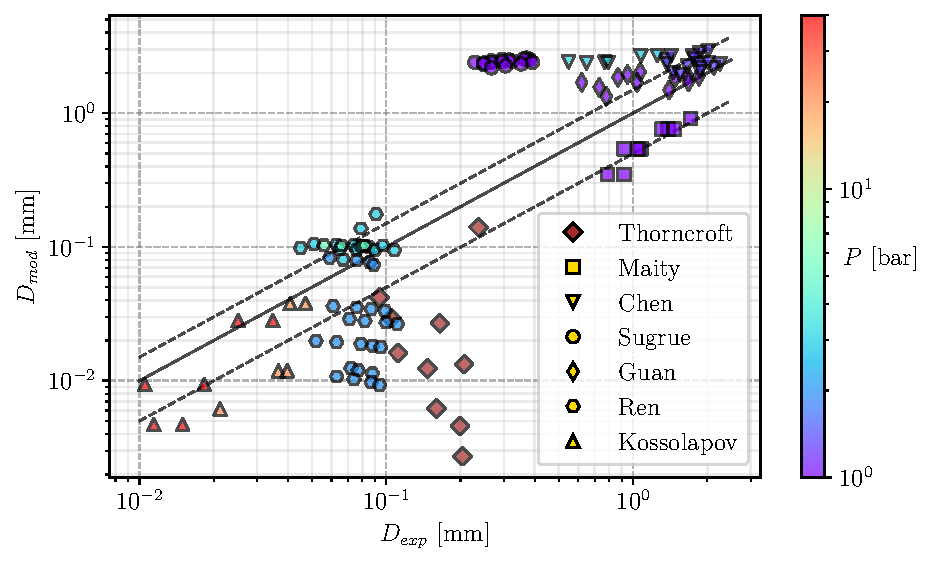
\includegraphics[width=0.7\textwidth]{img/forces/pred_nosensi.pdf}
}
\\
\subfloat[Mazzocco model]{
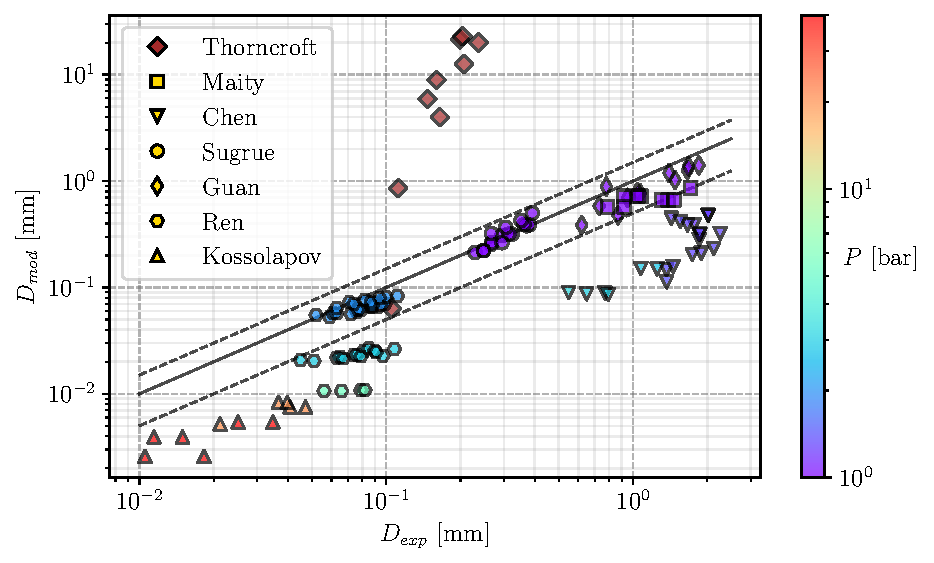
\includegraphics[width=0.7\textwidth]{img/forces/pred_mazzocco.pdf}
}

\caption{Predicted bubble departure diameters}
\label{fig:pred_nosensi}
\end{figure}




\subsection{Discussion and accounting for parameters uncertainties}


The aforementioned errors observed for the proposed model may originate from various reasons:

\begin{itemize}
\item The contact angle proposed for Sugrue cases is high with a large hysteresis, suggesting strongly deformed and flattened bubbles under the truncated sphere hypothesis. Based on images from Sugrue's work \cite{sugrue_experimental_2014}, a comparison between a real bubble with the assumed shape is presented on Figure \ref{fig:bubshape_sugrue}. This shows a huge difference which indicates that the contact angle and hysteresis values may be overestimated. Using the available images, the ratio of the bubble diameter to the apparent bubble foot would lead to an average contact angle $\theta \approx 20\degree$ for a truncated sphere. Noting that a larger inclination is observed for the bubbles under higher mass fluxes leads us to suppose a value $\dtheta \approx 15\degree$. This represent a similar inclination to contact angle ratio ($\dtheta / \theta$) compared to the initially proposed values. The resulting new shape is also presented on Figure \ref{fig:bubshape_sugrue} and seem to better represent the actual bubble.




\begin{figure}[h!]
\centering
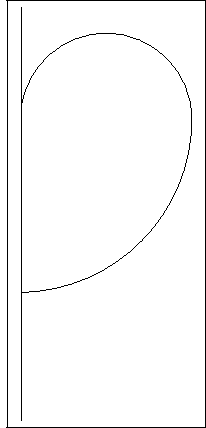
\includegraphics[height=0.4\linewidth]{img/forces/bub_sugrue.pdf}
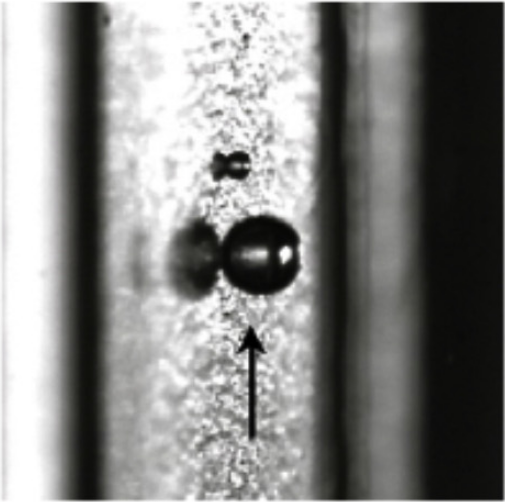
\includegraphics[width=0.45\linewidth]{img/forces/pic_sugrue.png}
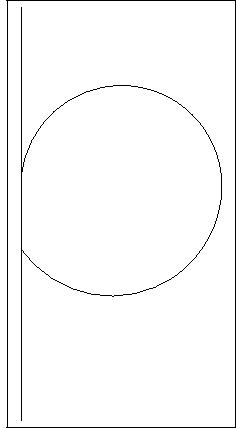
\includegraphics[height=0.4\linewidth]{img/forces/newbub_sugrue.pdf}
\caption{Initially assumed, real and reassessed bubble shape for Sugrue cases (picture adapted from \cite{sugrue_experimental_2014}).}
\label{fig:bubshape_sugrue}
\end{figure}


\item For cases where limited under and overestimation is observed, we may allow to account for an uncertainty as high as $5 \degree$ for the average contact angle $\theta$ and half-hysteresis $\dtheta$.

\item As mentioned earlier, applying the same contact angle and hysteresis over a wide range of measurements is a strong assumption, especially for cases where different pressures and bubble diameter variations are observed. Thus, we may slightly distinguish the applied values of $\theta$ and $\dtheta$ for different pressures within a given experiment, keeping a change no larger than $5 \degree$.

\item Kossolapov cases at $G_{L}=500~\debm$ are better predicted. Cases under higher mass fluxes ($1000$ and $1500~\debm$) present underestimation that could come from the value of $\dtheta$. At such mass fluxes, the Weber number can be up to a decade higher and bubbles may thus accept a larger inclination before detachment.

\item Cases of Ren and Chen rely on chosen values for $\theta$ and $\dtheta$ and not on measured ones. They are therefore subject to strong uncertainties. We can note that the values for Chen cases are significantly high.

\item The proposed growth law is still rather simple and may miss significant information, especially regarding bubble size and fluid properties such as the Prandtl number.

\item Errors on Thorncroft cases may be linked to uncertainties regarding FC-87 properties. Indeed, we use the values given at $T_{sat}=29\degree$ at 1 bar in his work \cite{thorncroft_experimental_1998}. However, the saturation temperature indicated in his test matrix is close to $40\degree$ which means that measurements were conducted at a higher pressure, for which we do not have FC-87 properties.


\end{itemize}





Therefore, using modified values of $\theta$ and $\dtheta$ among experimental data sets with no more than a $5 \degree$ change (except for Sugrue cases reassessed values) leads to predictions on Figure \ref{fig:pred_sensi}.






\begin{figure}[h!]

\subfloat[Modified contact angle and hysteresis values.]
{
\scriptsize
\centering
\begin{tabular}[b]{p{30mm}|c c } 
Author & $\theta$ [$\degree$] & $\dtheta$ [$\degree$]\\
\hline
\\
Thorncroft & 20 & 14 \\
\\
Maity & 45 & 10  \\
\\
Chen & 92.5 & 27.5 \\
\\
Sugrue & 20 & 15 \\
\\
Guan & 47.5 & 17.5 \\
\\
Ren (2 bar) & 45.5 & 8.5 \\
\\
Ren (3 bar) & 37.5 & 3.5 \\
\\
Ren (5 bar) & 35.5 & 3.5 \\
\\
Koss. (500$~\debm$) & 80 & 0.5 \\
\\
Koss. (1000$~\debm$) & 80 & 1 \\
\\
Koss. (1500$~\debm$) & 80 & 1.5 \\
\\
\hline
\end{tabular}

\label{tab:angle_sensi}
}
\subfloat[Predicted bubble departure diameters.]{
\centering
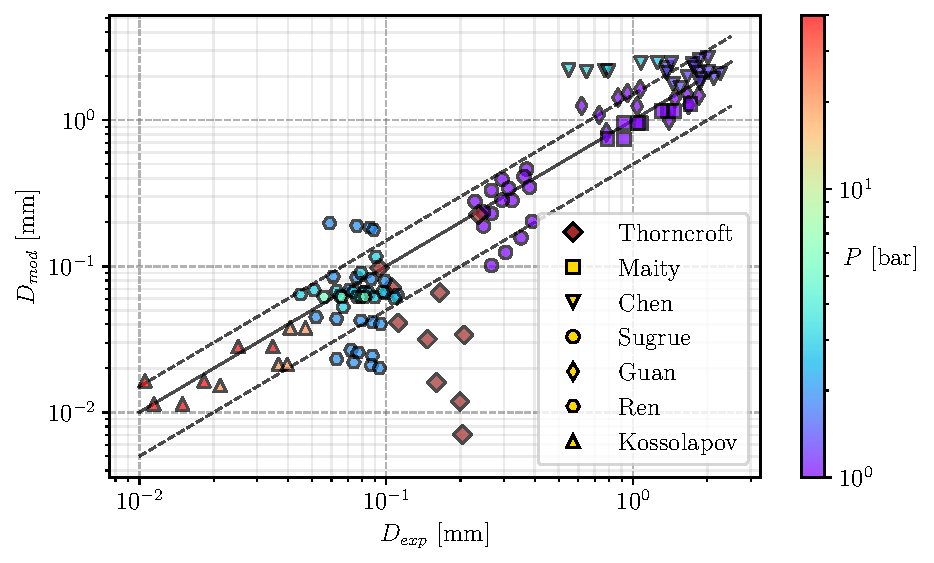
\includegraphics[width=0.7\textwidth]{img/forces/pred_sensi.pdf}
}

\caption{Proposed model performance while accounting for contact angle uncertainties}
\label{fig:pred_sensi}
\end{figure}



The predictive capacity of the model is significantly enhanced, especially on Sugrue's cases which tends to indicate that the contact angle reassessment was justified under the truncated sphere hypothesis. Table \ref{tab:mod_errors} summarizes the average errors obtained with the present model and Mazzoco's one.



\begin{table}[h!]

\scriptsize
\centering
\begin{tabular}[b]{p{30mm}|c c } 
Author & Mazzocco & Present model\\
\hline
\\
Thorncroft & 4874\% & 60.6\% \\
\\
Maity & 39.7\% & 13.8\%  \\
\\
Chen & 83.8\% & 69.9\% \\
\\
Sugrue & 9.73\% & 26.22\% \\
\\
Guan & 25.5\% & 36.8\% \\
\\
Ren & 40.32\% & 44.1\% \\
\\
Kossolapov & 78.3\% & 24.1\% \\
\\
Total & 442\% & 43\%\\
\\
Total \newline (without Thorncroft) & {46.58\%} & {41.4\%}\\
\hline
\end{tabular}
\caption{Average relative error reached by the models.}
\label{tab:mod_errors}
\end{table}


The proposed model achieves an overall better predictive capability even when excluding measurements from Thorncroft on which Mazzocco's model strongly overestimates the departure diameter. Mazzocco's model is still better on Sugrue and Guan cases since it was built and validated using those measurements. It better predicts results from Ren but only for the 2 bar cases while it underestimates the departure diameter for higher pressures. Those results are a coupled effect of his optimized growth law along with the imposed value of $r_{w}/R$ and the use of the inclination angle to hinder departure as mentioned in \ref{subsec:AM}.

The approach demonstrated the importance and the strong influence of the contact angle and hysteresis. A small change of their value (staying in the uncertainty range of $5\degree$) allowed to reach reasonable predictions over a large range of bubble departure diameters with the model of this paper, using a reduced number of empirical parameters.


\section{Sliding phase}\label{sliding}


\subsection{Modeling}

After departure, bubbles slide over a distance $l_{sl}$ which scales the impact of the sliding phenomenon over the wall heat transfer. Achieving good prediction of bubble sliding velocity is then important if one wishes to correctly quantify its impact. 

Following the force balance framework presented in Section \ref{sec:forces}, we can write Newton's second law parallel to the wall for the sliding bubble.


\begin{align}
\nonumber \rho_{V}\derive{\parth{V_{b}U_{b}}}{t} =& - \pi R\sigma f_{C,x}+ \frac{4}{3}\pi R^{3}\parth{\rho_{L}-\rho_{V}}g + \frac{1}{2}C_{D}\rho_{L}\pi R^{2} U_{L}^{2} \\
%
&+ \frac{4}{3}\pi R^{3}\rho_{L}\crocht{3C_{AM,x}\frac{\dot{R}}{R}U_{rel} - C_{AM,x}\derive{U_{b}}{t}}
\end{align}

This equation can be re-written to express the bubble acceleration.

\begin{align}
\nonumber \parth{1+\frac{\rho_{L}}{\rho_{V}}C_{AM,x}}\derive{U_{b}}{t} = & \parth{\frac{\rho_{L}}{\rho_{V}}-1}g + \frac{3}{8}\frac{C_{D}}{R}\frac{\rho_{L}}{\rho_{V}}\parth{U_{L}-U_{b}}\bars{U_{L}-U_{b}} \\
%
&+ 3\frac{\dot{R}}{R}\crocht{C_{AM,x}\frac{\rho_{L}}{\rho_{V}}\parth{U_{L}-U_{b}}-U_{b}} - \frac{3}{4}\frac{\sigma}{\rho_{V}}\frac{f_{C,x}}{R^{2}}
\label{eq:ub_dot}
\end{align}

Then, we numerically solve this equation from the moment when $R\geq R_{d}$ using a first order Euler scheme for a duration close to the experimental sliding time. Next sections compare obtained results against low and high pressure data.


\subsection{Low Pressure Sliding}

Maity \cite{maity_effect_2000} provided simultaneous measurements of bubble radius and velocity over time for three liquid mass fluxes in vertical boiling. To assess the validity of Eq.~\ref{eq:ub_dot}, we modify the growth constant $K$ in order to roughly match experimental radius measurements. The goal is to verify if the force balance allows a good prediction of bubble velocity provided a correct bubble growth. The contact angles were kept the same as in \ref{subsec:Dd_pred} since Maity provided average values over the bubble lifetime.

Results are displayed on Figure \ref{fig:slide_maity}. The model seems to fairly good predict bubble sliding velocity for the 3 cases. The moment of departure is a bit underestimated as previously observed (Figure \ref{fig:pred_nosensi}).

The biggest discrepancy is observed for the case at $G_{L}=143.8~ \debm$. The slope of the velocity profile is close to the experiments, but the bubble reaches a nearly constant acceleration too rapidly which yields an approximately constant overestimation of $0.1$~m/s.

The $G_{L}=239.6~ \debm$ is well predicted regarding the velocity. However, the growth profile was difficult to match since measurements exhibit significant changes in growth regime after departure, which is probably due to the bubble being large enough to be impacted by the bulk flow. A finer model for bubble growth could be of interest here.


We can note that values of $K$ between 0.5 and 1 were used to better fit the bubble radius time profile.




\begin{figure}[h!]
\begin{center}
\subfloat[$\Delta T_{w}=5.0$\degree C, $G_{L}=73.8~\debm$]{
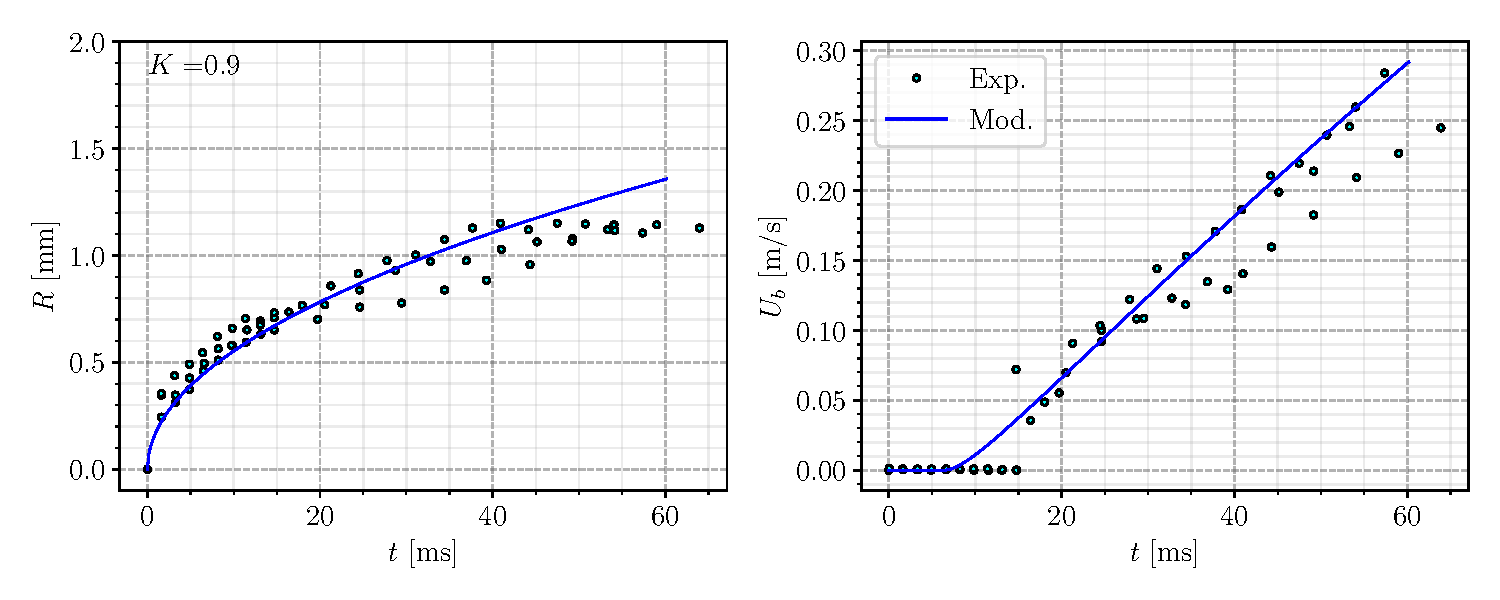
\includegraphics[width=0.9\linewidth]{img/forces/maity_V0p077.pdf}
} 
\\
\subfloat[$\Delta T_{w}=5.9$\degree C, $G_{L}=143.8~\debm$]{
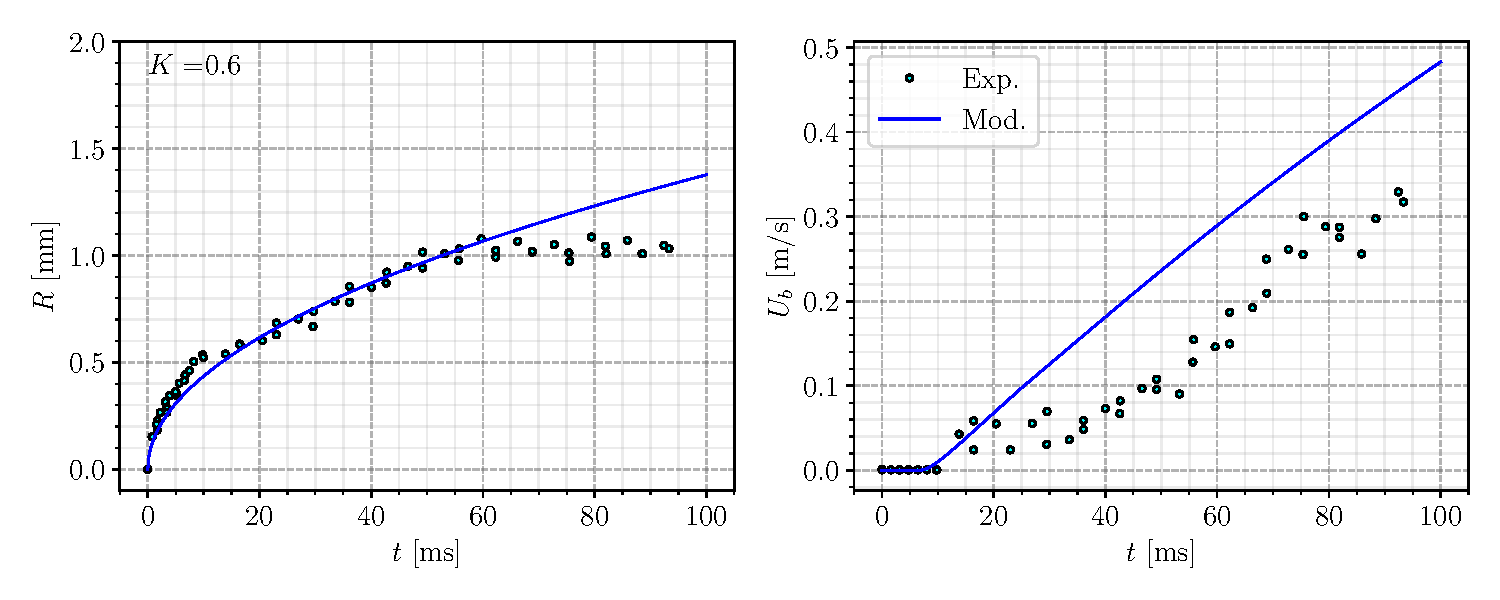
\includegraphics[width=0.9\linewidth]{img/forces/maity_V0p15.pdf}
}
\\
\subfloat[$\Delta T_{w}=5.9$\degree C, $G_{L}=239.6~\debm$]{
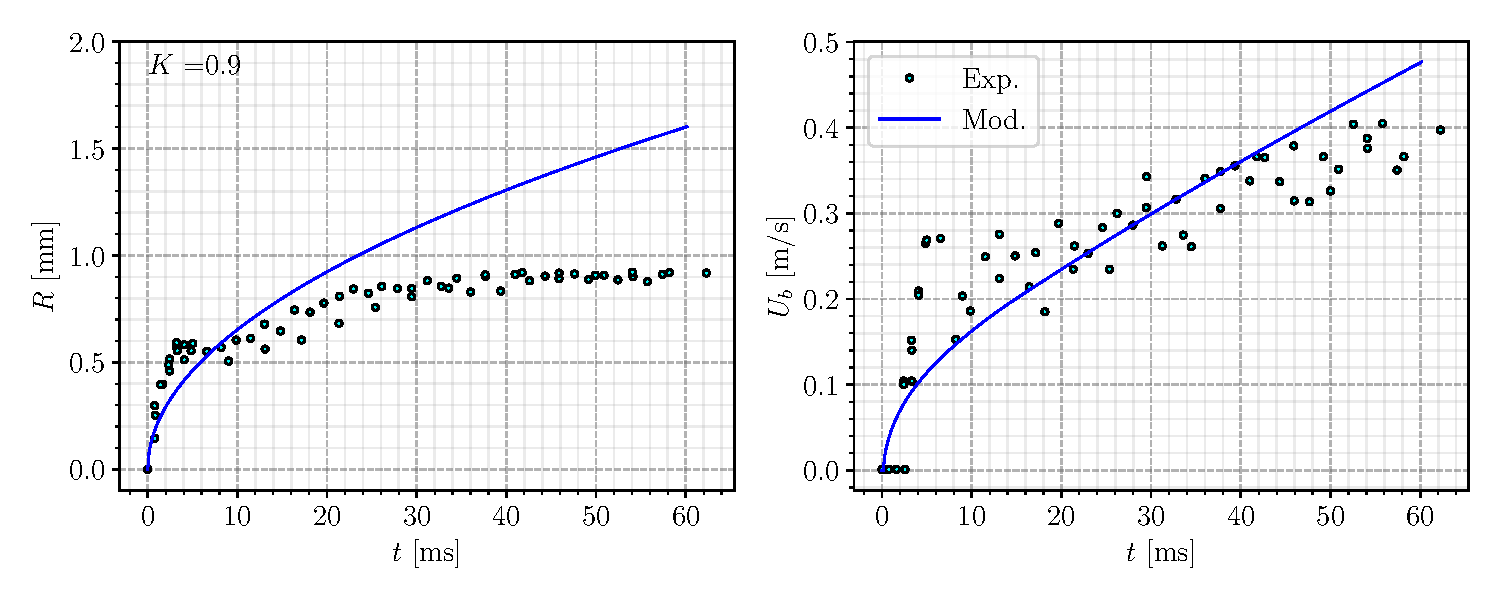
\includegraphics[width=0.9\linewidth]{img/forces/maity_V0p25.pdf}
}
	\caption{Bubble sliding velocity predictions on Maity cases}
	\label{fig:slide_maity}
\end{center}
\end{figure}





\subsection{High Pressure Sliding}

In his work, Kossolapov \cite{kossolapov_experimental_2021} conducted measurements of radius and sliding length over thousands of individual bubbles and then provided the associated statistical distributions. To compare our model with his measurements, we took the upper and lower bounds of $R$ and $l_{sl}$ over time and plotted the associated bands of measured values as shown on Figure \ref{fig:slide_koss_20bar} and \ref{fig:slide_koss_40bar}.


Comparisons were done for cases at 20 bar and 40 bar and 3 different values of $G_{L}$. The value of $\dtheta$ for the simulations was kept really small ($2 \degree$ at 20 bar and $0.5\degree$ at 40 bar) since bubble tilt is supposed to reduce during sliding because the relative velocity regarding the liquid flow is diminishing. Moreover, higher pressure means smaller bubbles that are even more unlikely to present a significant contact angle hysteresis. We also want to mention that neglecting the capillary term in Eq.~\ref{eq:ub_dot} had a minor impact over the results except that the bubble accelerates a little bit faster. 

The obtained results are in good agreement with the sliding length profile vs. time, which means bubble sliding velocity is well predicted for those cases.

Once the estimation of $\Delta T_{w}$ using Eq.~\ref{eq:frost} is corrected as mentioned in \ref{subsec:data_map}, values of $K$ between 0.8 and 1.3 reasonably fits the bubble radius measurements.






\begin{figure}[h!]
\begin{center}
\subfloat[$\phi_{w}=0.178$~MW/m\up{2}, $G_{L}=500~\debm$]{
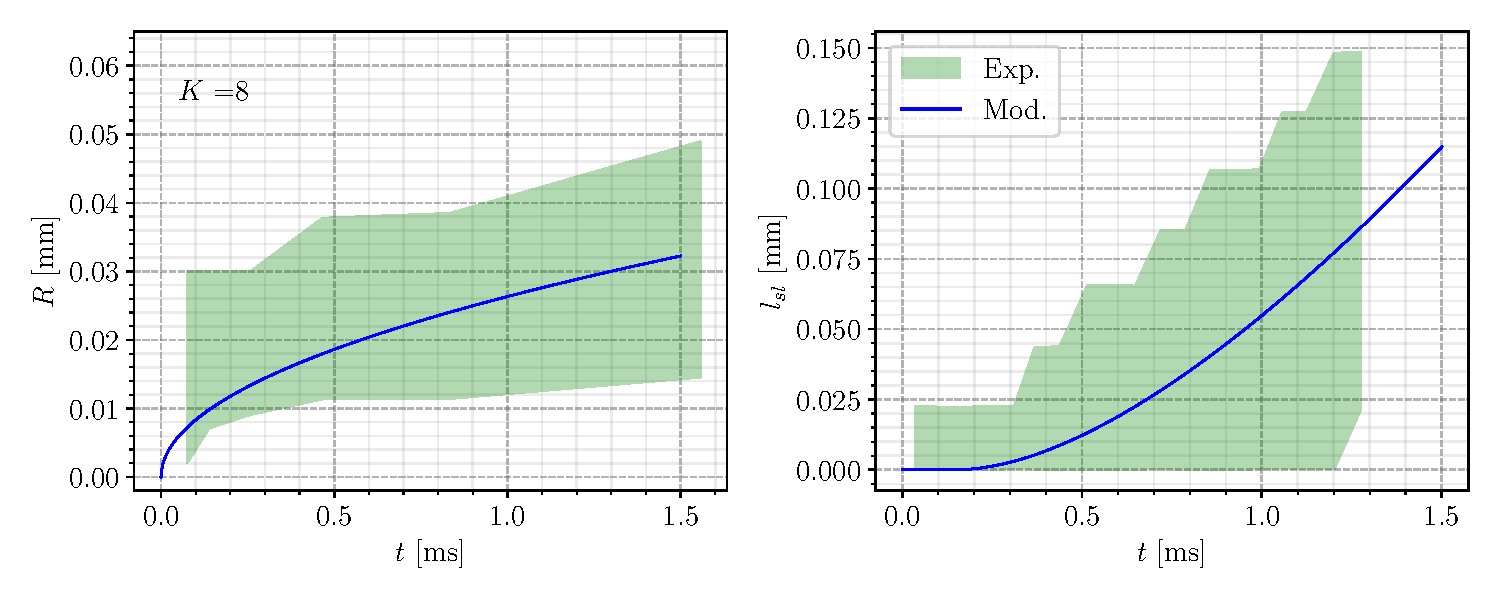
\includegraphics[width=0.9\linewidth]{img/forces/Koss_P20_G500.pdf}
} 
\\
\subfloat[$\phi_{w}=0.495$~MW/m\up{2}, $G_{L}=994~\debm$]{
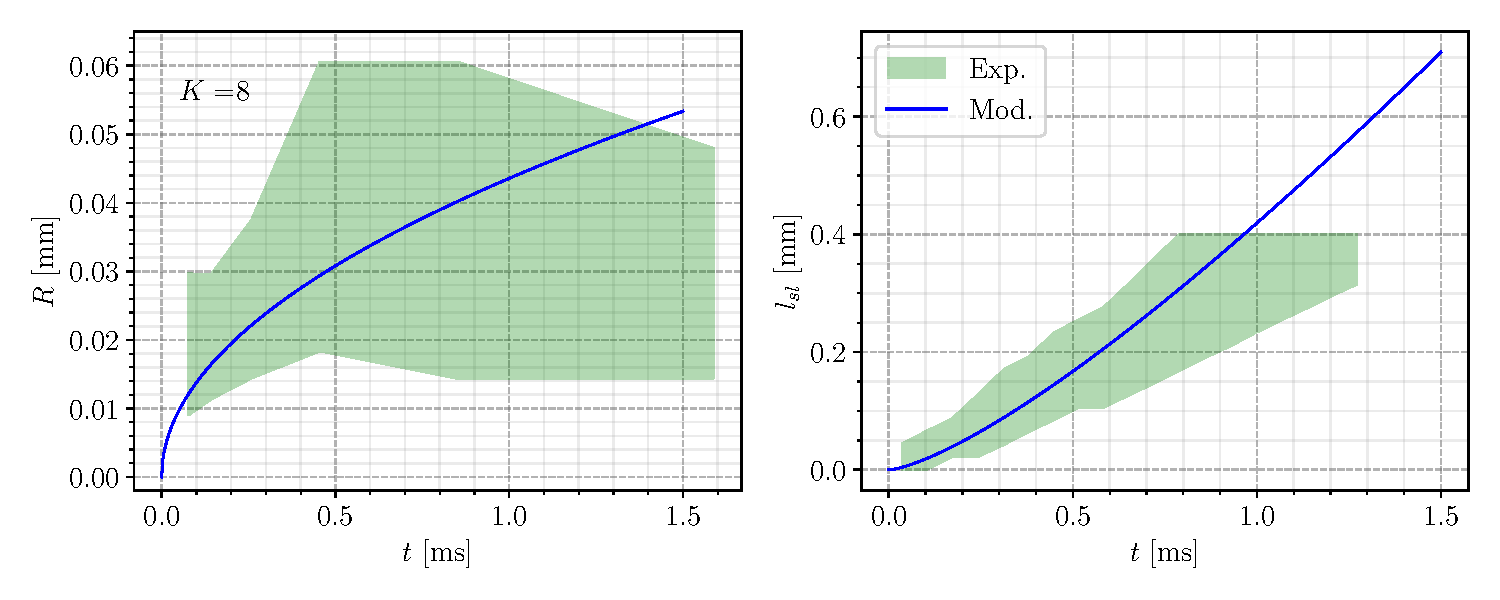
\includegraphics[width=0.9\linewidth]{img/forces/Koss_P20_G1000.pdf}
} 
\\
\subfloat[$\phi_{w}=0.487$~MW/m\up{2}, $G_{L}=1504~\debm$]{
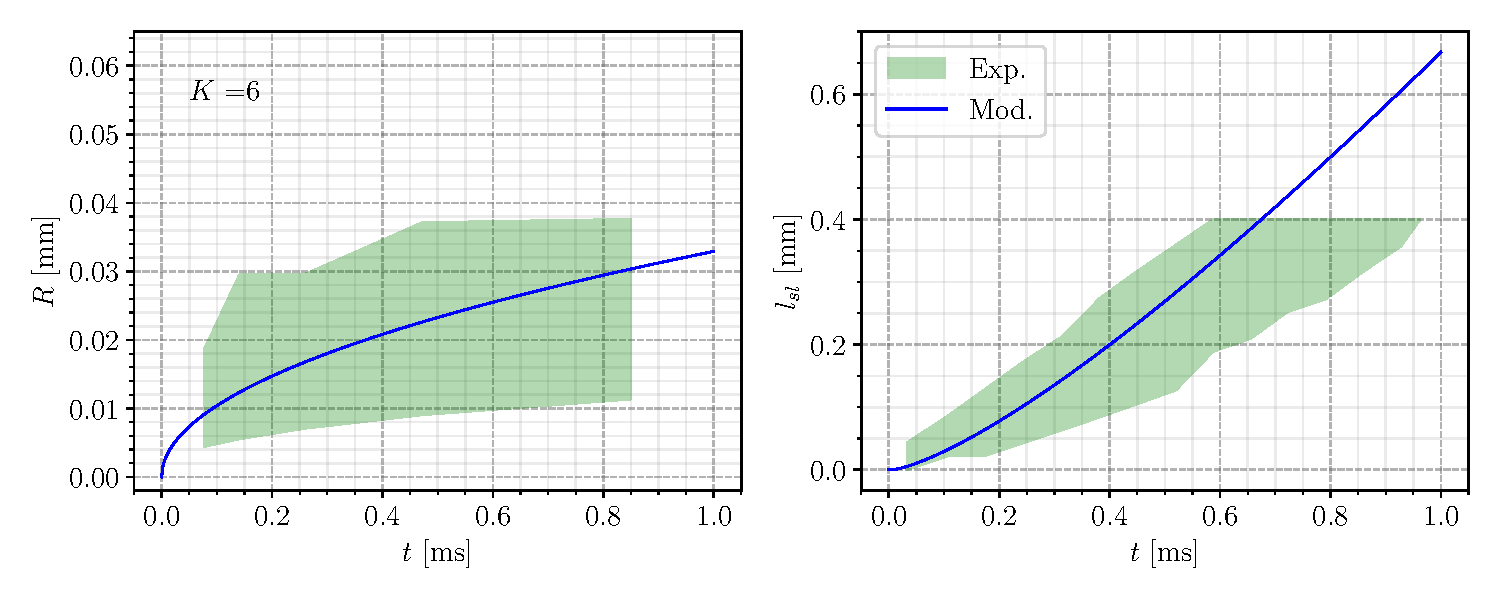
\includegraphics[width=0.9\linewidth]{img/forces/Koss_P20_G1500.pdf}
} 
	\caption{Bubble sliding length predictions on Kossolapov cases - $P=20$ bar}
	\label{fig:slide_koss_20bar}	
\end{center}
\end{figure}



\begin{figure}[h!]
\begin{center}
\subfloat[$\phi_{w}=0.291$~MW/m\up{2}, $G_{L}=500~\debm$]{
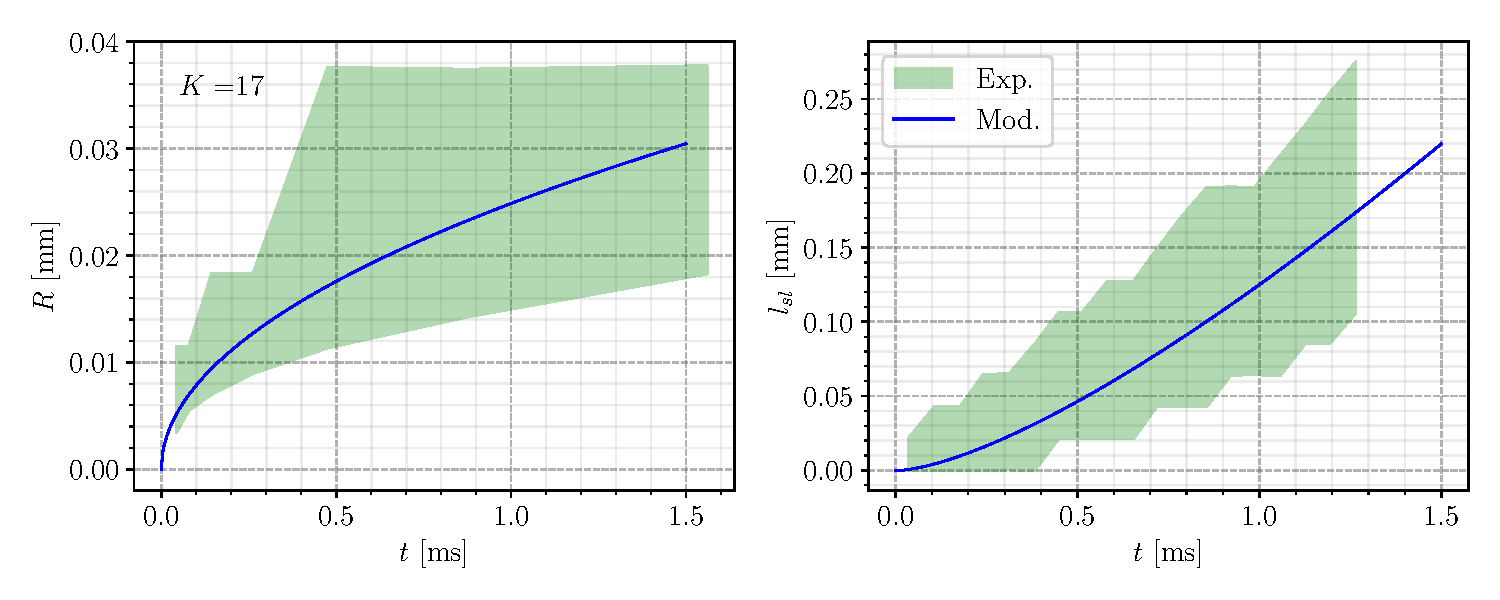
\includegraphics[width=0.9\linewidth]{img/forces/Koss_P40_G500.pdf}
} 
\\
\subfloat[$\phi_{w}=0.361$~MW/m\up{2}, $G_{L}=994~\debm$]{
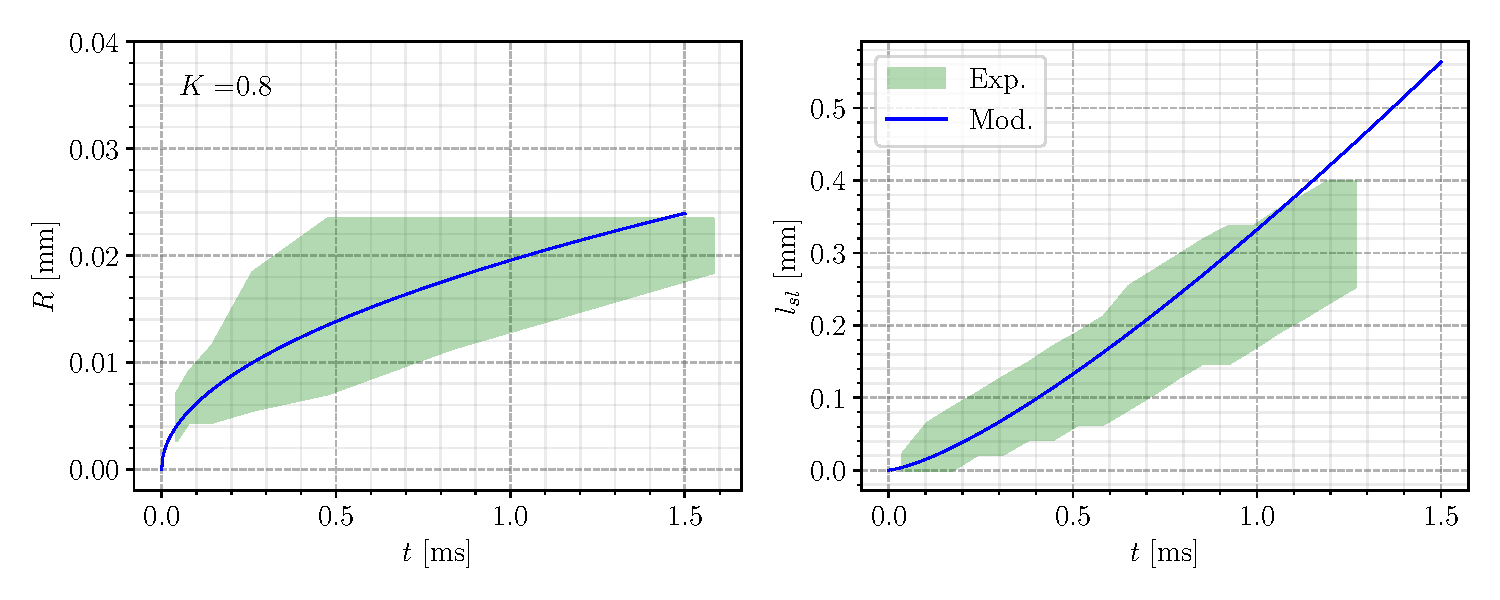
\includegraphics[width=0.9\linewidth]{img/forces/Koss_P40_G1000.pdf}
} 
\\
\subfloat[$\phi_{w}=0.613$~MW/m\up{2}, $G_{L}=1504~\debm$]{
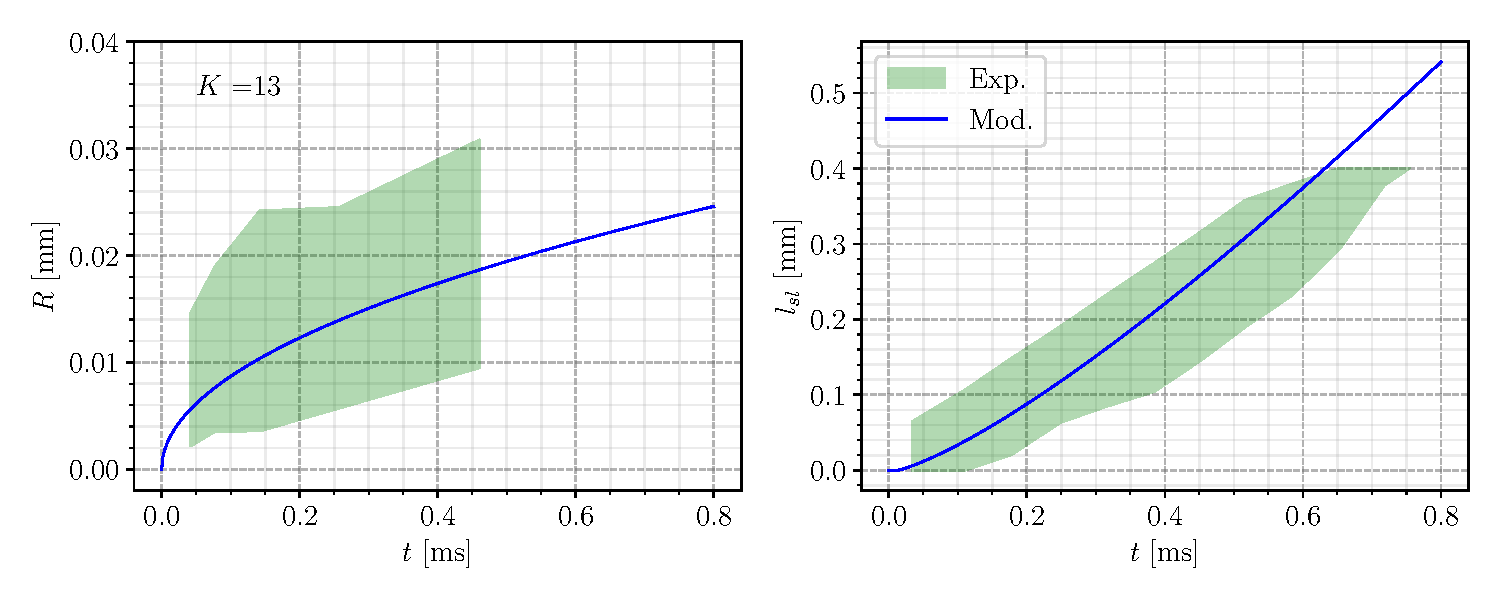
\includegraphics[width=0.9\linewidth]{img/forces/Koss_P40_G1500.pdf}
} 
	\caption{Bubble sliding length predictions on Kossolapov cases - $P=40$ bar}	
	\label{fig:slide_koss_40bar}
\end{center}
\end{figure}




\section{Conclusion}\label{ccl}

In this work, we proposed a revisited force balance for a single bubble in a vertical upward boiling flow. This force balance was then used to study bubble departure by sliding and compared with bubble departure diameter and sliding velocity measurements. The main highlights of this study are:

\begin{itemize}
\item The use of a recent correlation to compute the Drag coefficient thanks to DNS results of Shi \etal \cite{shi_drag_2021}.
\item Reassessed computation of the Added Mass force and associated coefficients from the expression of the liquid kinetic energy proposed by Van Der Geld \cite{van_der_geld_dynamics_2009}. 
\item A global force balance that avoids including extra empirical parameters. We notably get rid of empirical choices regarding bubble foot radius and do not include an arbitrary bubble inclination angle to create an Added Mass term hindering departure.
\item A non dimensional approach leading to force regime maps to qualitatively determine the dynamic regime in which bubbles are departing from the nucleation site. It shows that the detaching Added Mass term due to external liquid flow is rarely negligible and often dominates at low pressure. Increasing pressure mostly leads to Drag dominant regimes.
\item Bubble departure diameter predictions are achieved with a reasonable accuracy over a large range of measured values from 7 data sets. This could be reached by accepting an uncertainty of $5 \degree$ for the values of the contact angle $\theta$ and half-hysteresis $\dtheta$ to which the model was sensitive. This indicates that using fixed values for large data sets seems incorrect and that extra empiricism may not be needed if a proper modeling of those parameters was achieved.
\item Bubble sliding velocity simulations showed a good agreement with experimental observations both at low and high pressure provided a correct bubble growth profile.
\end{itemize}


The limitations of the developed approach lie mainly in the simple and empirical law to estimate the growth constant $K$ (Eq. \ref{eq:Kgrowth}). This could be enriched by a clean modeling of the bubble growth including effects such as condensation, microlayer evaporation and impact of the external liquid flow. Existing models rely on empirical values which thus reduces their general applicability outside of their validation range. For instance, studies conducted by Zhou \cite{zhou_experimental_2020} and Yoo \cite{yoo_development_2018} could be used by enriching their modeling with finer results to get rid of data fitting. DNS results such as those regarding bubble growth in a flowing superheated or subcooled liquid by Legendre \etal \cite{legendre_thermal_1998} could be of interest in that prospect.


Finally, the precise estimation of the contact angle and hysteresis remains a critical parameter to predict departure by sliding as demonstrated throughout this study. Local measurements of those values and their evolution with operating conditions would be a very valuable information in that regard. The article of Song \& Fan \cite{song_temperature_2021} that sums up existing modeling and experimental measurements provides a good overview of the problem and identifies the associated challenges that are still to be tackled.




\section{Bubble Lift-Off}


